\documentclass[10pt]{beamer}\usepackage[]{graphicx}\usepackage[]{color}
%% maxwidth is the original width if it is less than linewidth
%% otherwise use linewidth (to make sure the graphics do not exceed the margin)
\makeatletter
\def\maxwidth{ %
  \ifdim\Gin@nat@width>\linewidth
    \linewidth
  \else
    \Gin@nat@width
  \fi
}
\makeatother

\definecolor{fgcolor}{rgb}{0.345, 0.345, 0.345}
\newcommand{\hlnum}[1]{\textcolor[rgb]{0.686,0.059,0.569}{#1}}%
\newcommand{\hlstr}[1]{\textcolor[rgb]{0.192,0.494,0.8}{#1}}%
\newcommand{\hlcom}[1]{\textcolor[rgb]{0.678,0.584,0.686}{\textit{#1}}}%
\newcommand{\hlopt}[1]{\textcolor[rgb]{0,0,0}{#1}}%
\newcommand{\hlstd}[1]{\textcolor[rgb]{0.345,0.345,0.345}{#1}}%
\newcommand{\hlkwa}[1]{\textcolor[rgb]{0.161,0.373,0.58}{\textbf{#1}}}%
\newcommand{\hlkwb}[1]{\textcolor[rgb]{0.69,0.353,0.396}{#1}}%
\newcommand{\hlkwc}[1]{\textcolor[rgb]{0.333,0.667,0.333}{#1}}%
\newcommand{\hlkwd}[1]{\textcolor[rgb]{0.737,0.353,0.396}{\textbf{#1}}}%
\let\hlipl\hlkwb

\usepackage{framed}
\makeatletter
\newenvironment{kframe}{%
 \def\at@end@of@kframe{}%
 \ifinner\ifhmode%
  \def\at@end@of@kframe{\end{minipage}}%
  \begin{minipage}{\columnwidth}%
 \fi\fi%
 \def\FrameCommand##1{\hskip\@totalleftmargin \hskip-\fboxsep
 \colorbox{shadecolor}{##1}\hskip-\fboxsep
     % There is no \\@totalrightmargin, so:
     \hskip-\linewidth \hskip-\@totalleftmargin \hskip\columnwidth}%
 \MakeFramed {\advance\hsize-\width
   \@totalleftmargin\z@ \linewidth\hsize
   \@setminipage}}%
 {\par\unskip\endMakeFramed%
 \at@end@of@kframe}
\makeatother

\definecolor{shadecolor}{rgb}{.97, .97, .97}
\definecolor{messagecolor}{rgb}{0, 0, 0}
\definecolor{warningcolor}{rgb}{1, 0, 1}
\definecolor{errorcolor}{rgb}{1, 0, 0}
\newenvironment{knitrout}{}{} % an empty environment to be redefined in TeX

\usepackage{alltt}
\usetheme{metropolis}           % Use metropolis theme

\usepackage{graphicx}

\DeclareGraphicsExtensions{.pdf,.jpeg,.jpg,.png}

\usepackage{subcaption}
\usepackage{amsmath}

\usepackage{tikz}
\usetikzlibrary{bayesnet}
\usepackage{pgfplots}
\pgfplotsset{compat=1.13}

\usepackage[framemethod=TikZ, xcolor=RGB]{mdframed}
\definecolor{mydarkblue}{rgb}{0,.06,.5}
\definecolor{mydarkred}{rgb}{.5,0,.1}
\definecolor{myroyalblue}{rgb}{0,.1,.8}
\mdfdefinestyle{MyFrame}{%
    linecolor=mydarkblue,
    outerlinewidth=0.5pt,
    roundcorner=2pt,
    innertopmargin=2pt,
    innerbottommargin=2pt,
    innerrightmargin=2pt,
    innerleftmargin=2pt,
    backgroundcolor=blue!10}

\newcommand{\Rbb}{\mathbb{R}}
\newcommand{\Expect}{\mathbb{E}}
\newcommand{\Expecthat}{\hat{\mathbb{E}}}
\newcommand{\Var}{\text{Var}}
\newcommand{\Cov}{\text{Cov}}
\newcommand{\vbfamily}{\mathcal{Q}}
\newcommand{\etaopt}{\eta^{*}}
\newcommand{\etazopt}{\eta_z^{*}}
\newcommand{\etathetaopt}{\eta_\theta^{*}}
%\newcommand{\qopt}{q^{*}}
\newcommand{\targethat}{\hat{g}}
\newcommand{\QExpect}
{\Expect_{q\left(\theta, z \vert \eta_\theta, \etazopt(\eta_\theta)\right)}}
\newcommand{\atzero}{\Big\rvert_{\eta_\theta = \etathetaopt, \epsilon = 0}}
\newcommand{\etathetalin}{\eta_\theta^{LIN}}
\DeclareMathOperator*{\argmin}{arg\,min}





\title{Evaluating Sensitivity to the Stick Breaking Prior in
Bayesian Nonparametrics}
\date{November 17, 2020}
\author{Runjing (Bryan) Liu}
\institute{University of California, Berkeley}

\setbeamertemplate{Collaborators}[none]
\IfFileExists{upquote.sty}{\usepackage{upquote}}{}
\begin{document}
\maketitle

\begin{frame}{Collaborators}
  	\vspace{1em}
  	\begin{figure}
  		\begin{subfigure}{.4\textwidth}
  			\centering
  			
\includegraphics[height=2cm]{collaborators/bryan}
        \captionsetup{justification=centering}
  			\caption*{Runjing (Bryan) Liu \\ UC Berkeley}
  		\end{subfigure}%
  		\begin{subfigure}{.4\textwidth}
  			\centering
  			
\includegraphics[height=2cm]{collaborators/ryan}
  			\caption*{Ryan Giordano \\ MIT}
  		\end{subfigure}\\ \vspace{0.11in}
      \begin{subfigure}{.4\textwidth}
  			\centering
  			
\includegraphics[height=2cm]{collaborators/mike}
  			\caption*{Michael I.\ Jordan \\ UC Berkeley}
  		\end{subfigure}%
  		\begin{subfigure}{.4\textwidth}
  			\centering
  			
\includegraphics[height=2cm]{collaborators/tamara}
  			\caption*{Tamara Broderick \\ MIT}
  		\end{subfigure}\\
  	\end{figure}

\end{frame}


\begin{frame}{Motivating Example}

Inferring population structure from genomic sequences.
\begin{itemize}
  \item[--] Genetic data from Taita thrush, an endangered bird species native to Kenya
  \citep{galbusera:2000:thrush}
  %{\color{blue} \href{https://web.stanford.edu/group/pritchardlab/publications/pdfs/Pritch%ardEtAl00.pdf}{(Pritchard et al. 2000)}}
  \item[--] Microsatellites sequences of 155 individuals at 7 loci.
\end{itemize}


\begin{figure}[!h]
\centering
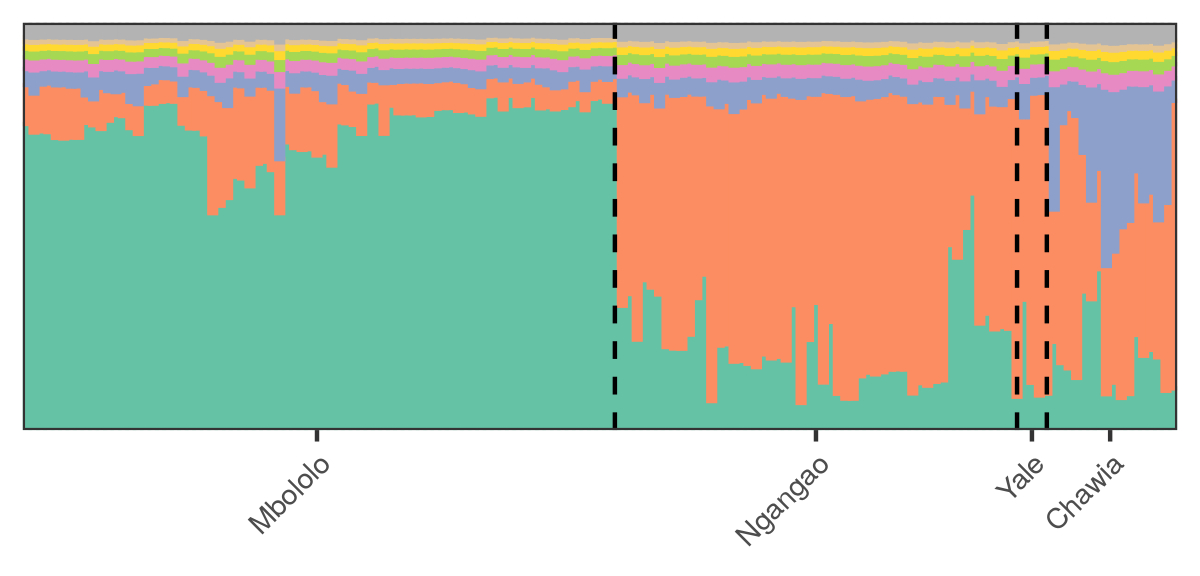
\includegraphics[width = 0.9\textwidth]{./figure/structure_init-1.png}
\end{figure}

\end{frame}

\begin{frame}{Motivating Example}

\begin{figure}[ht!]
\centering
\only<1-2>{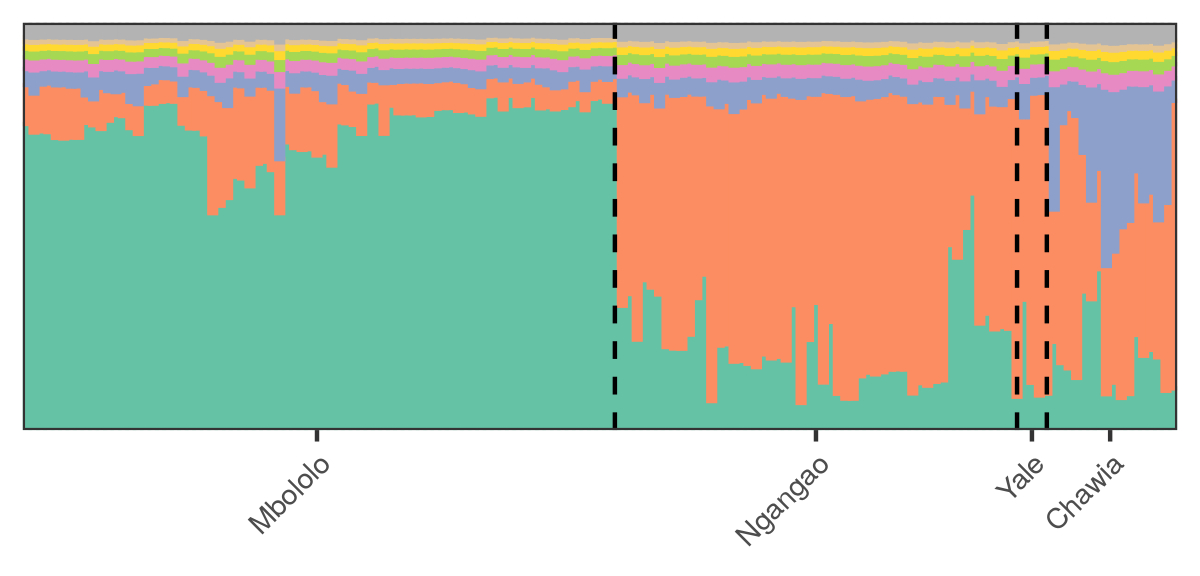
\includegraphics[width = 0.9\textwidth]{./figure/structure_init-1.png}}
\only<3>{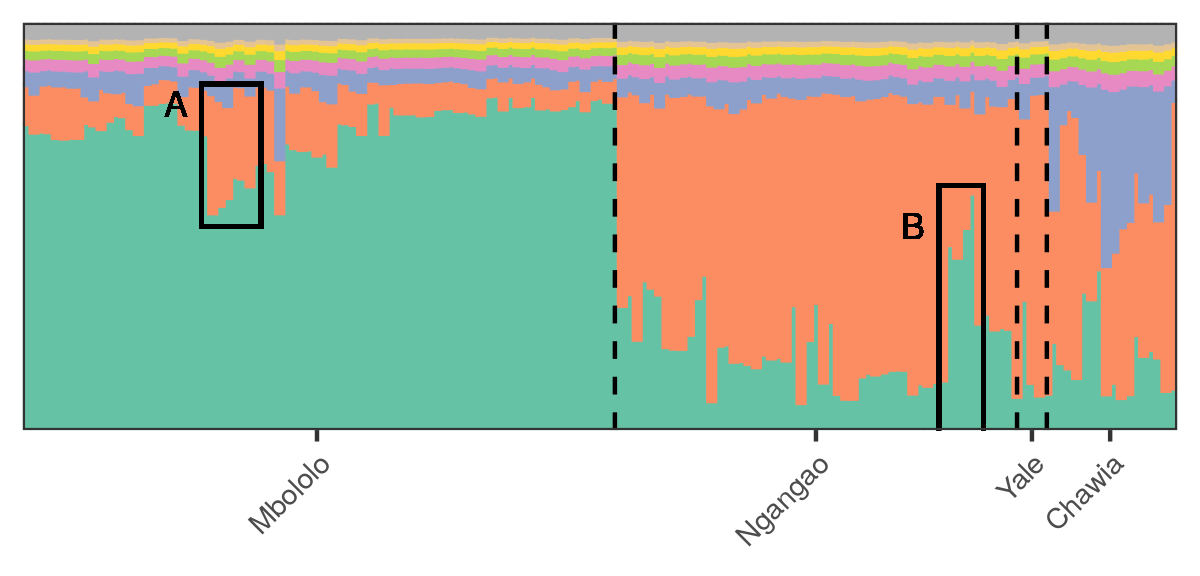
\includegraphics[width = 0.9\textwidth]{./figure/structure_migration-1.png}}
\end{figure}
\vspace{-1em}

%%%%%%%%%%%%%
% how many latent populations?
%%%%%%%%%%%%%
\only<1>{
%\textbf{How many latent populations (clusters) are present in the data set?}

- Three primary populations
{\large
\textcolor{pop1}{$\blacksquare$}
\textcolor{pop2}{$\blacksquare$}
\textcolor{pop3}{$\blacksquare$}
}.

- Many small, rare populations
{\large 
\textcolor{pop4}{$\blacksquare$}
\textcolor{pop5}{$\blacksquare$}
\textcolor{pop6}{$\blacksquare$}
\textcolor{pop7}{$\blacksquare$}
\textcolor{pop8}{$\blacksquare$}
}. 

{\bf Question: How many distinct populations (clusters) are there...}
\vspace{-0.5em}
\begin{itemize}
    \item ...in this dataset?
    \item ...with more than $N$ loci?
    \item ...in a future dataset of the same size?
\end{itemize}
\vspace{3.5em}
}



%%%%%%%%%%%%%
% coclustering
%%%%%%%%%%%%%
\only<2-3>{
Individuals are generally clustered by geographic locations:
\begin{minipage}{0.3\textwidth}
 Mbololo $\approx$ {\large \textcolor{pop1}{$\blacksquare$}}
\end{minipage}
\begin{minipage}{0.3\textwidth}
 Ngangao $\approx$ {\large \textcolor{pop2}{$\blacksquare$}}
\end{minipage}
\begin{minipage}{0.35\textwidth}
Chawia $\approx$
    {\large 
    \textcolor{pop1}{$\blacksquare$} + 
    \textcolor{pop2}{$\blacksquare$} + 
    \textcolor{pop3}{$\blacksquare$}}
\end{minipage}

\textbf{Question: Which individuals cluster together?}

Exceptions to the clustering give evidence of historical migrations.
}

\only<2> {
% so that the figure aligns across the \only ....
% is there a better way to do this?
\vspace{2em}
}
\only<3>{
For example, the groups of individuals in A and B suggest migration
between the Mbololo and Ngangao locations. 
}
\end{frame}



\begin{frame}{Motivating Example}
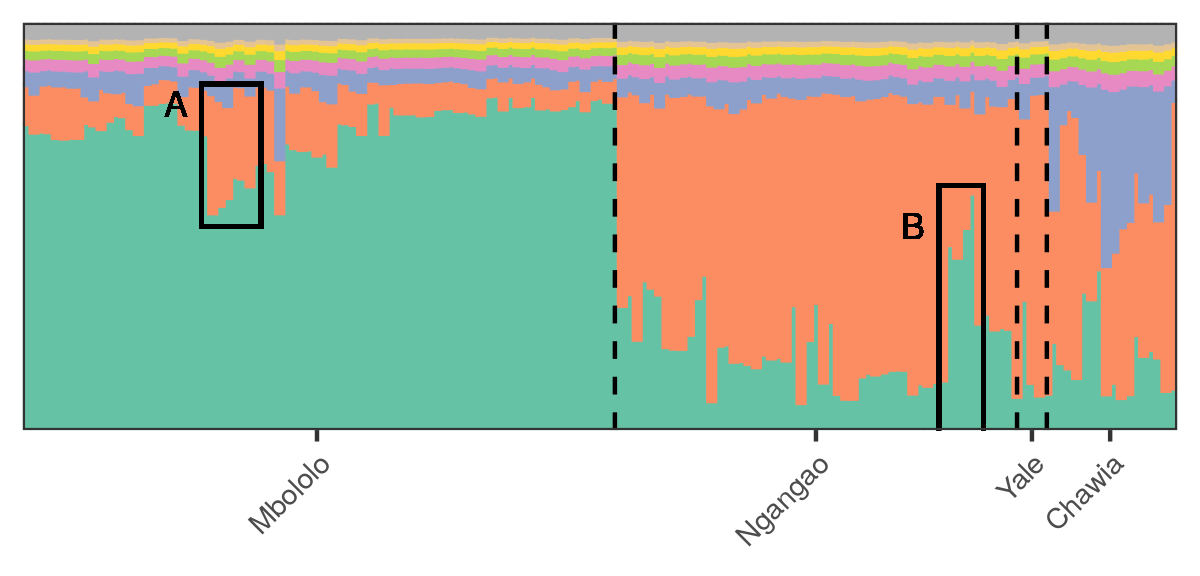
\includegraphics[width = 0.9\textwidth]{./figure/structure_migration-1.png}

How many distinct clusters are there?
%
Which individuals cluster together?

A \textbf{discrete Bayesian nonparametric (BNP)} model makes these questions 
amenable to Bayesian inference...

...but the answer may depend on the \textbf{prior you choose.}

\end{frame}


\begin{frame}{Motivating Example}

\begin{figure}[!h]
\centering
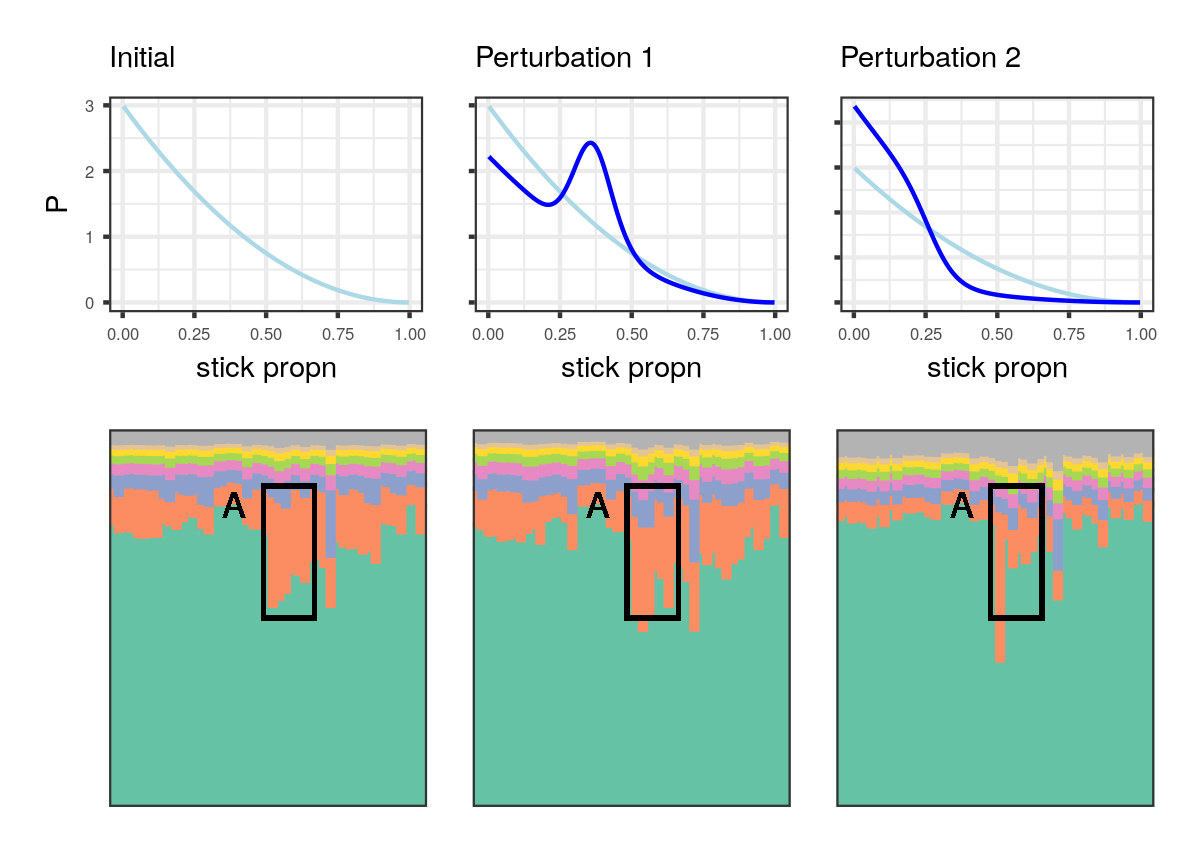
\includegraphics[width = \textwidth]{./figure/mbololo_motivating_ex-1.png}
\end{figure}

\end{frame}



\begin{frame}{Research Problem}

A discrete Bayesian nonparametric (BNP) model makes scientific
questions amenable to Bayesian inference.

\pause

We approximate the exact posterior using variational Bayes (VB).

\pause

\textbf{Question}: How sensitive is the VB approximation, and the resulting
inferences, to BNP model choices?

\pause

\textbf{Problem}: Re-running VB for multiple model choices is expensive.

\pause

\textbf{We propose}: A linear approximation to efficiently
estimate BNP sensitivity from a single run of VB.  The linear approximation
can both:
\begin{itemize}
    \item Provide approximate sensitivity with no refitting, or
    \item Guide the choice of priors for refitting.
\end{itemize}

\end{frame}



\begin{frame}{Outline}
\begin{itemize}
\item The BNP model
\vspace{0.1in}

\item The variational approximation
\vspace{0.1in}

\item Hyperparameter sensitivity
\vspace{0.1in}

\item Functional sensitivity and influence functions
\vspace{0.1in}

\item Results on population genetics modeling of the Taita thrush
\vspace{0.1in}

\end{itemize}
\end{frame}


\begin{frame}{The BNP Model \citep{sethuraman:1994:constructivedp}}
A {\bf Dirichlet process prior} allows for an infinite number of components.
\vspace{-0.2em}
\begin{figure}[!h]
\centering
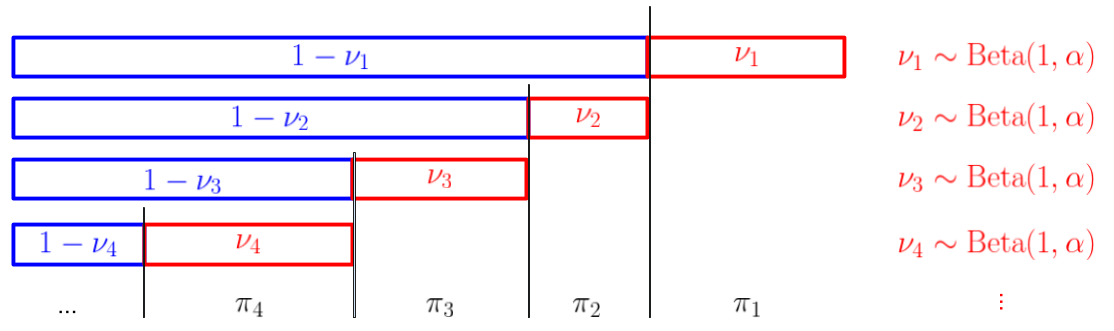
\includegraphics[width = 0.95\textwidth]{./static_figures/DP_stick_breaking.png}
\caption{A schematic of the Dirichlet process prior}
\end{figure}
\vspace{-0.2in}

While there are an infinite number of {\bf components}, there are a finite number of {\bf clusters} in a given dataset. 
%\pause 

Posterior quantities depend on the BNP prior, which is defined 
by the density of the stick-breaking process $\nuk \sim \p(\nuk)$.


% \begin{enumerate}[(1)]
% \item How many clusters are in the {\itshape current} dataset?

% %\pause
% \item How many clusters would we expect to see in a {\itshape new} dataset?
% \item Which observations in the current dataset cluster together?

% \end{enumerate}

% \pause

% These quantities depend on the choice of stick-breaking prior.

%\pause

\vspace{1em}

\begin{mdframed}[style=MyFrame]
\begin{center}
{\bf If $\nuk \sim \betadist{1, \alpha}$ what should $\alpha$ be?\\}
{\bf Why should $\p(\nuk)$ even be in the Beta family?}
\end{center}
\end{mdframed}

\end{frame}


\begin{frame}{The Variational Approximation}

Let $\theta$ be unknown parameters and $y$ the data.

We posit a class of mean-field distributions parameterized by a real vector $\eta$.

We solve
\begin{align*}
  \eta^* = \argmin_{\eta} KL\left(
      q(\theta \vert \eta )\big\| p(\theta | y)
      \right)
\end{align*}

\only<1>{
\begin{figure}[!h]
\centering
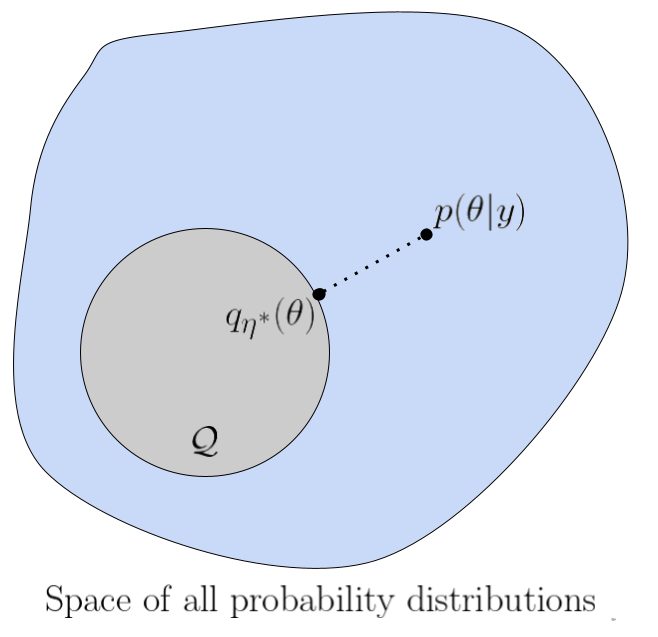
\includegraphics[width = 0.4\textwidth]{./figures/vi_schematic2.png}
\end{figure}
}

\only<2->{
Note that

\begin{itemize}
\item The optimal variational parameters $\eta^*$ depend on the prior through optimizing the KL objective.

\pause

\item The approximate posterior quantities are then functions of $\eta^*$, e.g.\
\begin{align*}
\eta^* \mapsto
\Expect_{q_{\eta^*}} \left[ \#\text{clusters} \right]
\quad \text{ or } \quad
\eta^* \mapsto
\Expect_{q_{\eta^*}}
\left[\#\{\substack{\text{clusters in}\\\text{new dataset}}\} \right].
\end{align*}

\end{itemize}
}

\only<3>{
\begin{mdframed}[style=MyFrame]
\begin{center}
{\bf How do these approximate posterior quantities depend on the DP prior?}
\end{center}
\end{mdframed}
}
\end{frame}


\begin{frame}{Hyperparameter Sensitivity}

Let $\t$ be some real-valued hyperparameter for the stick-breaking density.
%(For example, $\t$ could be $\alpha$, or parameterize a functional shape).  
\pause

Write $\etaopt(\t) := \argmin_{\eta} \KL{\eta, \t} = \argmin_{\eta} \KL{\q(\zeta \vert \eta) || \p(\zeta \vert \x, \t)}$.
\pause

{\bf Problem:} Evaluating $\etaopt(\t)$ requires solving a new optimization problem.
\pause

%\pause

{\bf We propose: } Approximate $\etaopt(\t)$ with a first-order
Taylor expansion:

\begin{align*}
  \etaopt(\t)  &\approx  
  %\etalin(\t) := 
  \etaopt(0) + \fracat{d \etaopt(\t)}{d \t}{\t=0} \t. 
\end{align*}
%
\pause
%
\vspace{-0.5em}
\begin{itemize}
\item<5-> We need only use a linear approximation for the map $\t \mapsto \etaopt(\t)$. We can retain nonlinearities in the map 
$\etaopt \mapsto \expect{\q(\zeta \vert \etaopt)}{\#\text{clusters}}
$, etc.
\vspace{0.5em}
\item<6-> This is ``Bayesian local robustness'' for VB \citep[cf.][]{gustafson:1996:local}
\vspace{0.5em}
\item<7-> The derivative can be evaluated using the implicit function theorem
and modern
{\color{blue} \href{https://jax.readthedocs.io/en/latest/}{automatic differentiation}}.
\end{itemize}
\end{frame}







\begin{frame}{Computing the Derivative \citep{giordano:2018:covariances}}

\textbf{Theorem 1.} (The derivative $d\etaopt(\t) / d\t$.)  

\onslide<2-> {
Define $\etaopt = \etaopt(0)$, $\hessopt := \fracat{\partial^2 \KL{\eta}}
                {\partial \eta \partial \eta^T}
                {\etaopt}$ and 
$\lqgrad{\nu \vert \etaopt} :=
    \fracat{\log \q(\nu \vert \etaopt)}{\partial \eta}{\etaopt}$.
}

\onslide<3->Assume:
\begin{itemize}
    \item<3-> The Hessian at the optimum, $\hessopt$, is non-singular. %\pause
    \item<4-> The optimal VB parameters, $\etaopt$, are interior. %\pause
    \item<5-> We can exchange limits and $\q$ expectations as needed in a 
        neighborhood of $\etaopt$ and $\t=0$.  %\pause
    \begin{itemize}
        %\item Dominated convergence theorem on a laundry list of functions.
        \item This imposes some regularity conditions on the prior $\p(\nu \vert \t)$.
    \end{itemize}
\end{itemize}

\onslide<6->{
Then the map $\t \mapsto \etaopt(\t)$ is continuously
differentiable at $\t=0$ with
%
\begin{align*}
%
\fracat{d \etaopt(\t)}{d \t}{0} ={}&
    - \hessopt^{-1}
    \expect{\q_{\etaopt}}{
        \lqgrad{\nu \vert \etaopt}
        \fracat{\partial \log \p(\nu \vert \t)}{\partial \t}{\t=0}
    }.
%
\end{align*} \hfill $\square$
}

\onslide<7->{
{\bf Note:} The computation of $\hessopt^{-1}$ is the computationally 
difficult part.  For our BNP problem, $\hessopt$ is sparse.
}

\end{frame}

\begin{frame}{A Simple Example: Iris Data}

We fit a Gaussian mixture model with a DP prior to
the iris data.

\begin{figure}[!h]
  \centering
  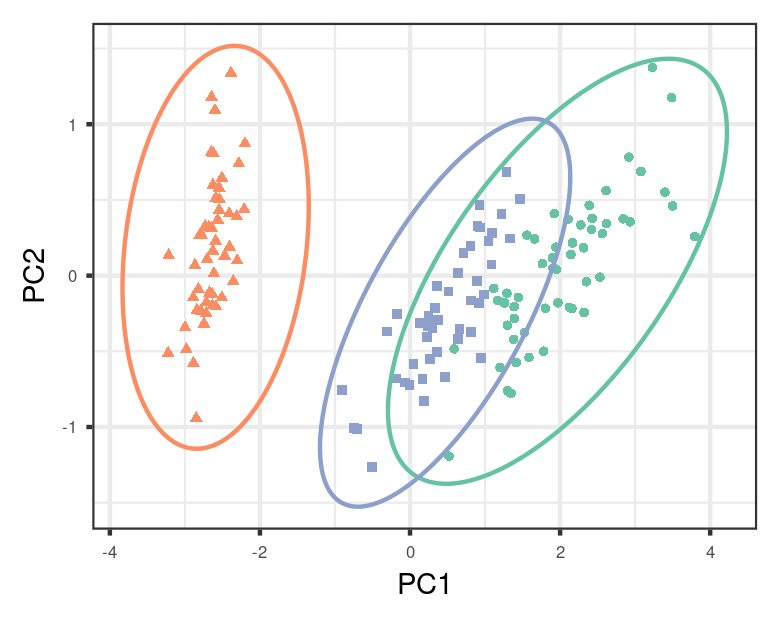
\includegraphics[width = 0.6\textwidth]{./figure/iris_init-1.png}
  \caption*{The iris data in principal component space and GMM fit at $\alpha = 6$.}
\end{figure}

\end{frame}

\begin{frame}{Iris Data: Parametric Sensitivity}

\begin{figure}[!h]
  \only<1>{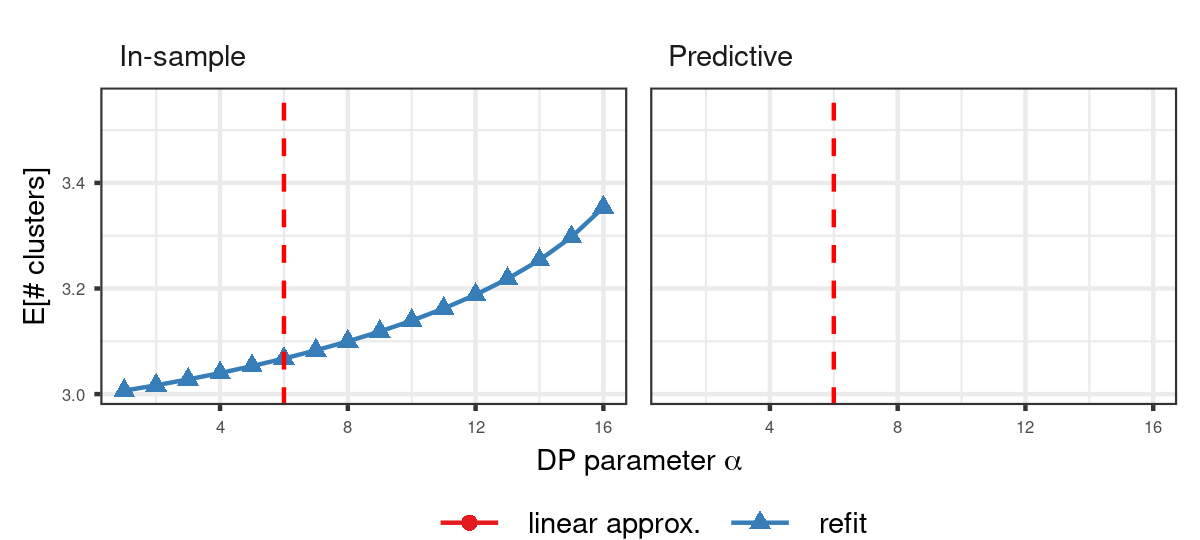
\includegraphics[width = \textwidth]{./figure/iris_alphasens_refit-1.png}}%
  \only<2>{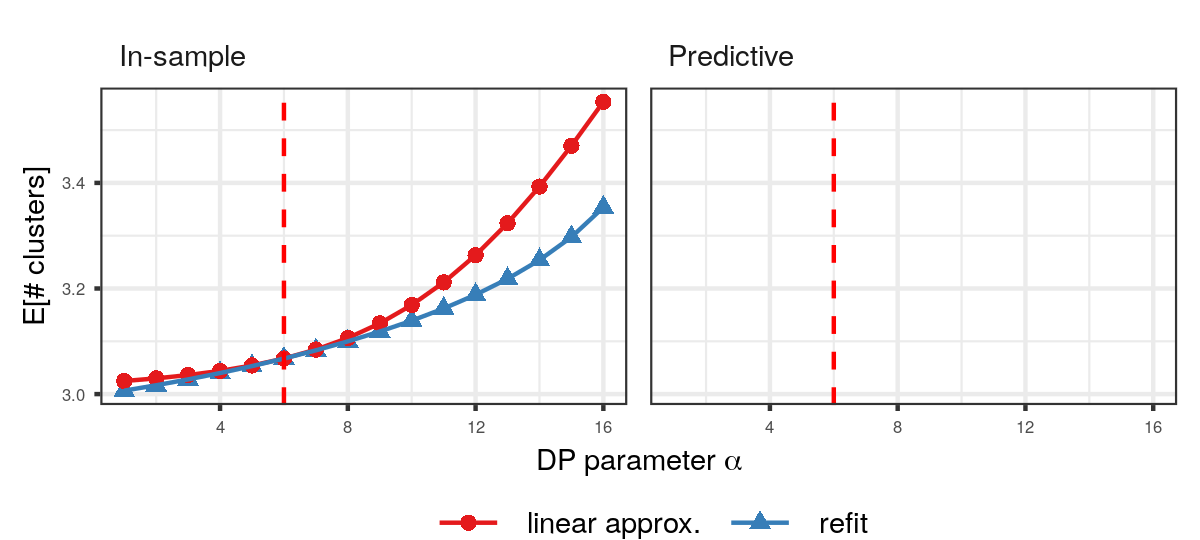
\includegraphics[width = \textwidth]{./figure/iris_alphasens_insample-1.png}}%
  \only<3>{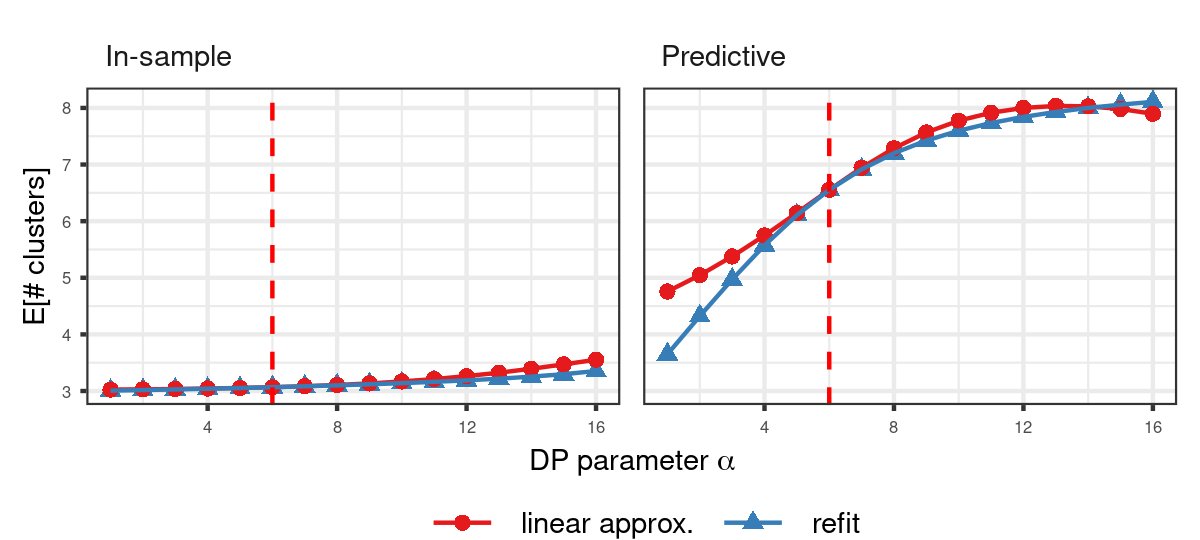
\includegraphics[width = \textwidth]{./figure/iris_alphasens_all-1.png}}
  \caption*{The expected number of posterior clusters in the iris data as $\alpha$ varies.}
\end{figure}

\end{frame}


\begin{frame}{A simple example: iris data}

We fit a Gaussian mixture model with a Bayesian non-parametric prior to
the iris data.

\begin{figure}[!h]
  \centering
  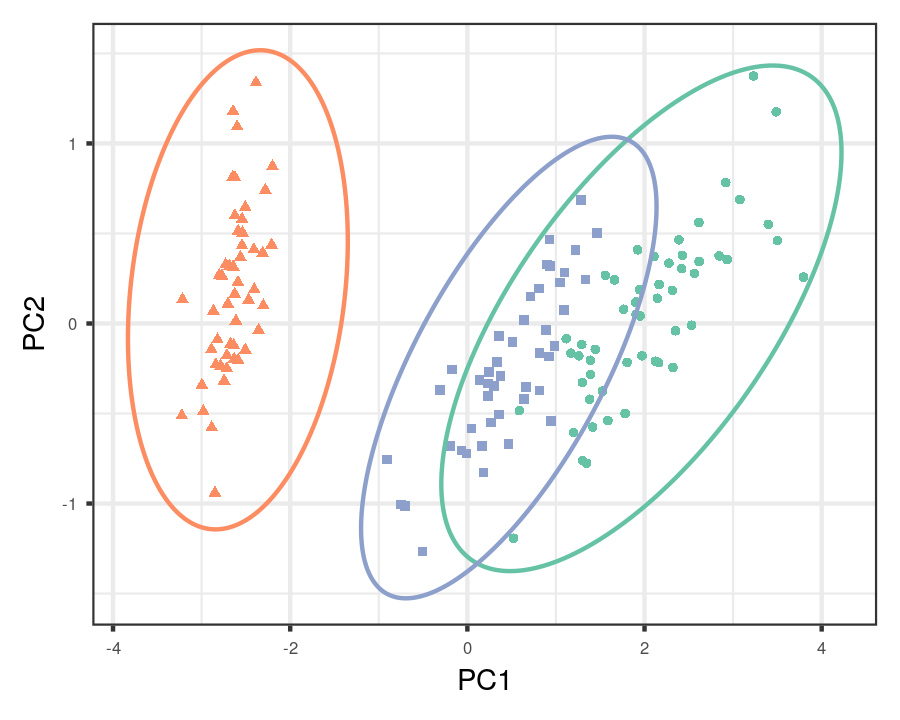
\includegraphics[width = 0.6\textwidth]{./figures/iris_init_fit.png}
  \caption*{The iris data in principal component space and GMM fit at $\alpha = 6$.}
\end{figure}

\end{frame}

\begin{frame}{iris data: parametric sensitivity}
  \begin{figure}[!h]
    \centering
    \only<1>{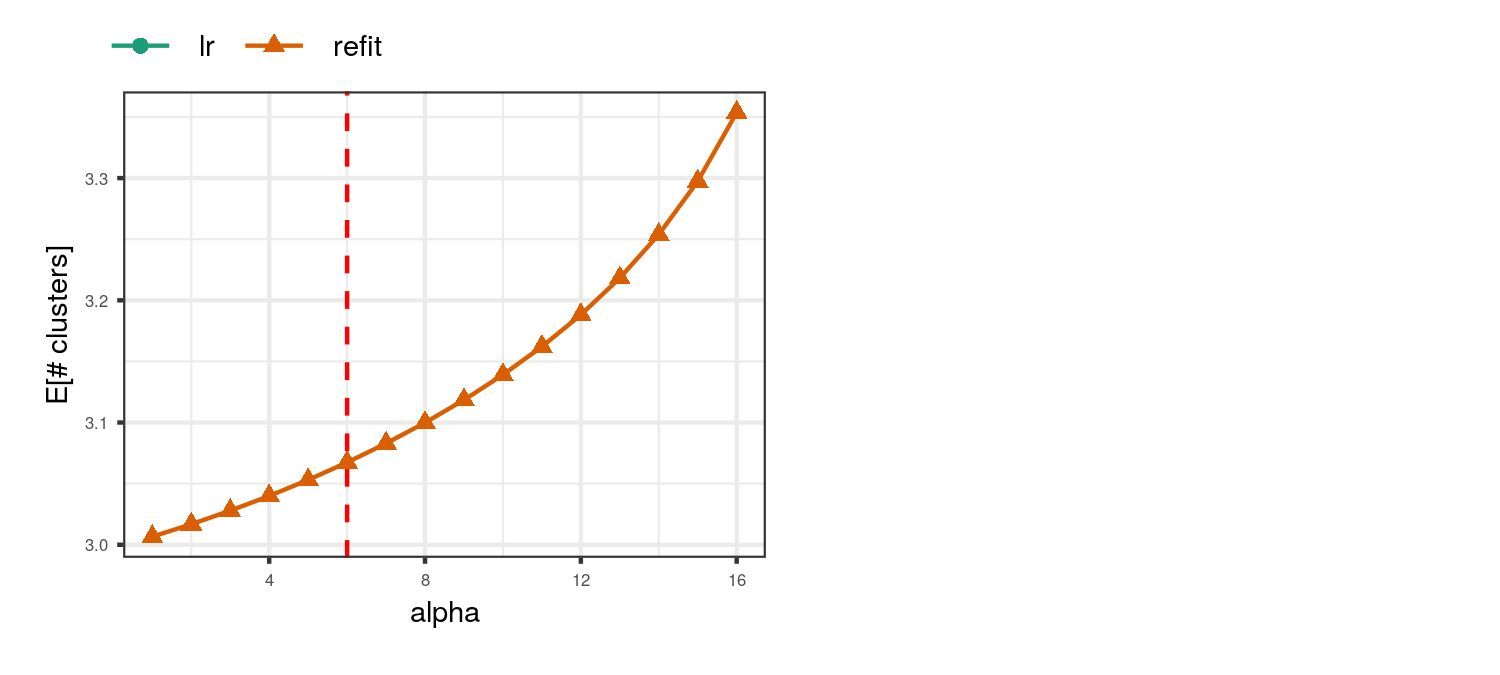
\includegraphics[width = \textwidth]{./figures/iris_alpha_sens0.png}}
    \only<2>{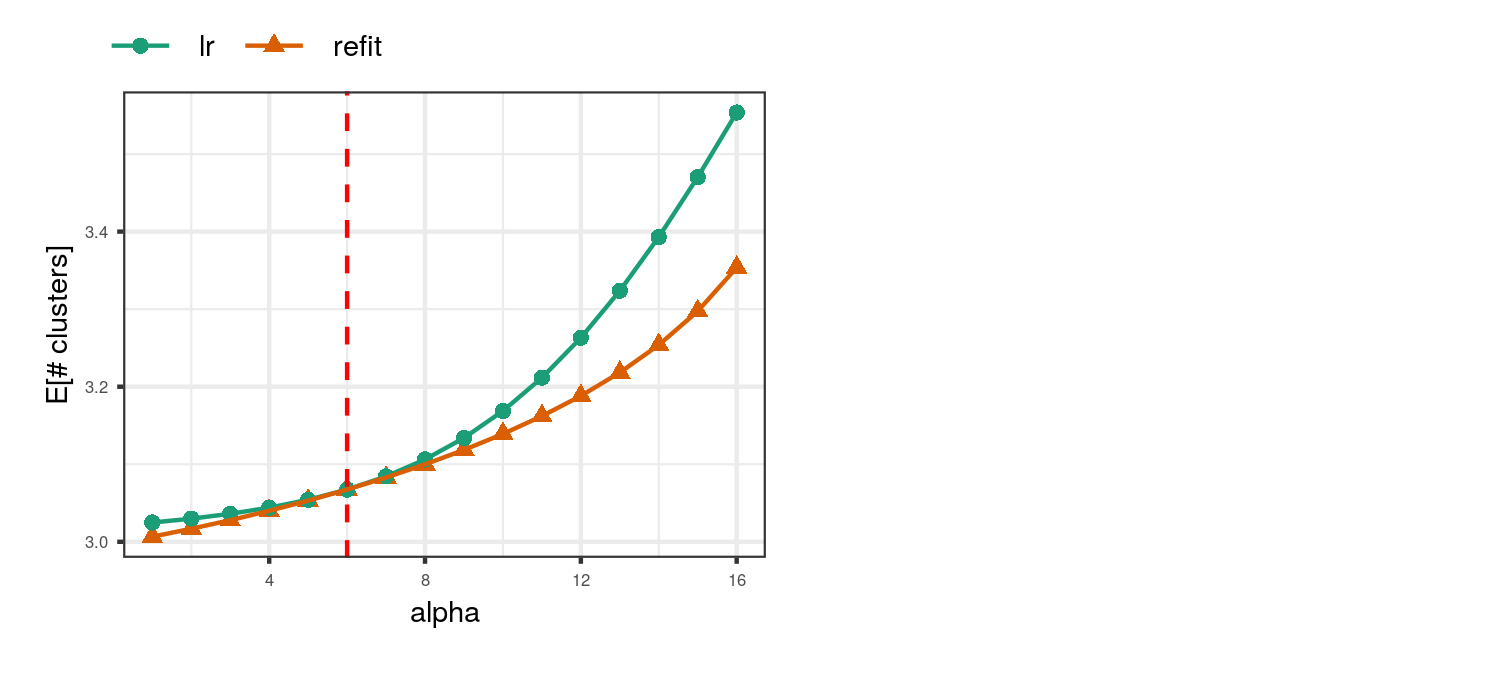
\includegraphics[width = \textwidth]{./figures/iris_alpha_sens1.png}}
    \only<3>{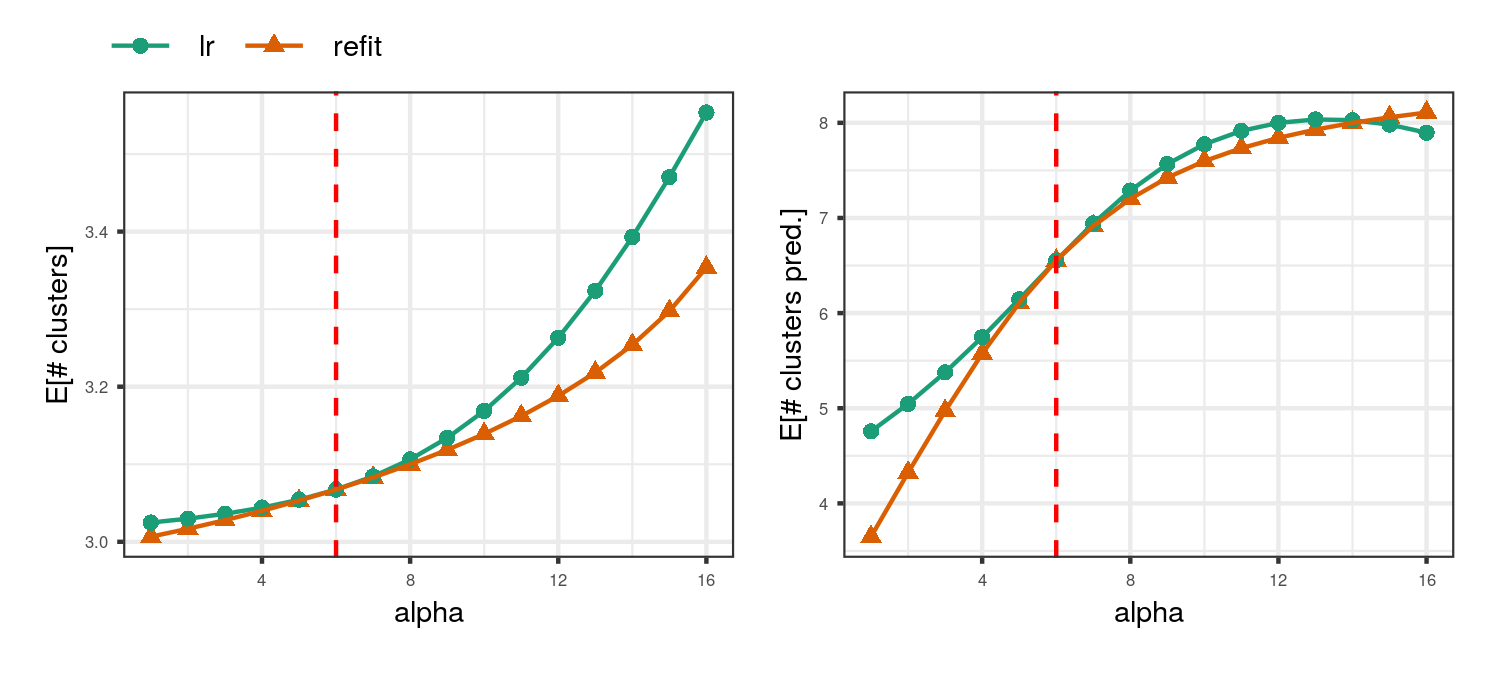
\includegraphics[width = \textwidth]{./figures/iris_alpha_sens2.png}}
    \caption*{The expected number of posterior clusters in the iris data as $\alpha$ varies.}
  \end{figure}

\end{frame}

\begin{frame}{iris data: influence functions}
  \begin{figure}[!h]
    \centering
    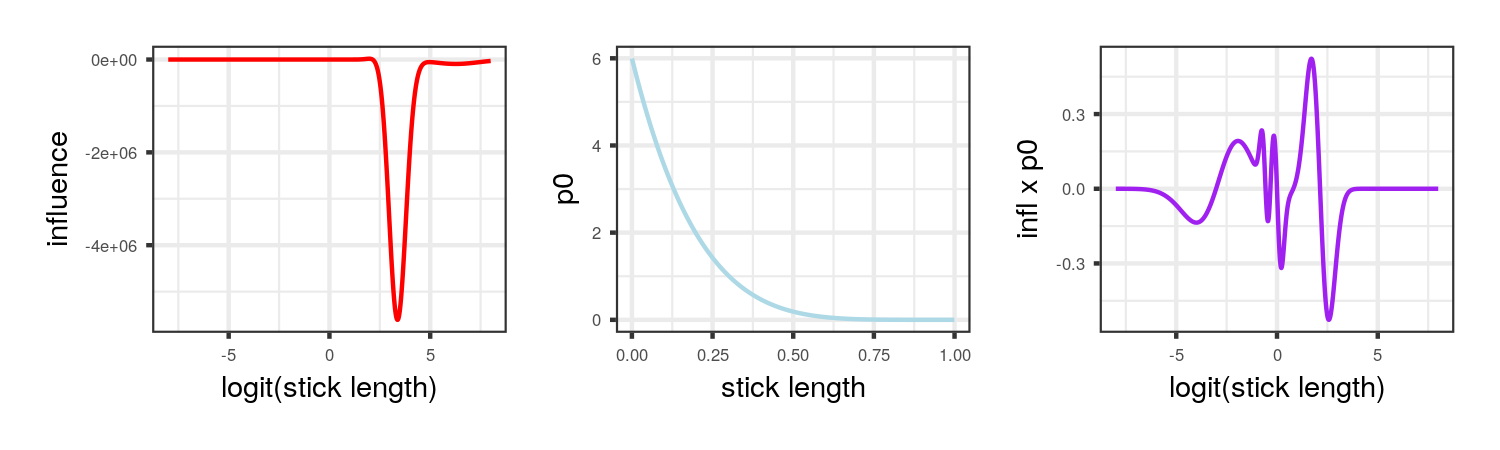
\includegraphics[width = \textwidth]{./figures/iris_influence_function.png}
    \caption*{The influence function of the expected number of predicted clusters.}
\end{figure}
\end{frame}

\begin{frame}{iris data: functional perturbations}
  \begin{figure}[!h]
    \centering
    \only<1>{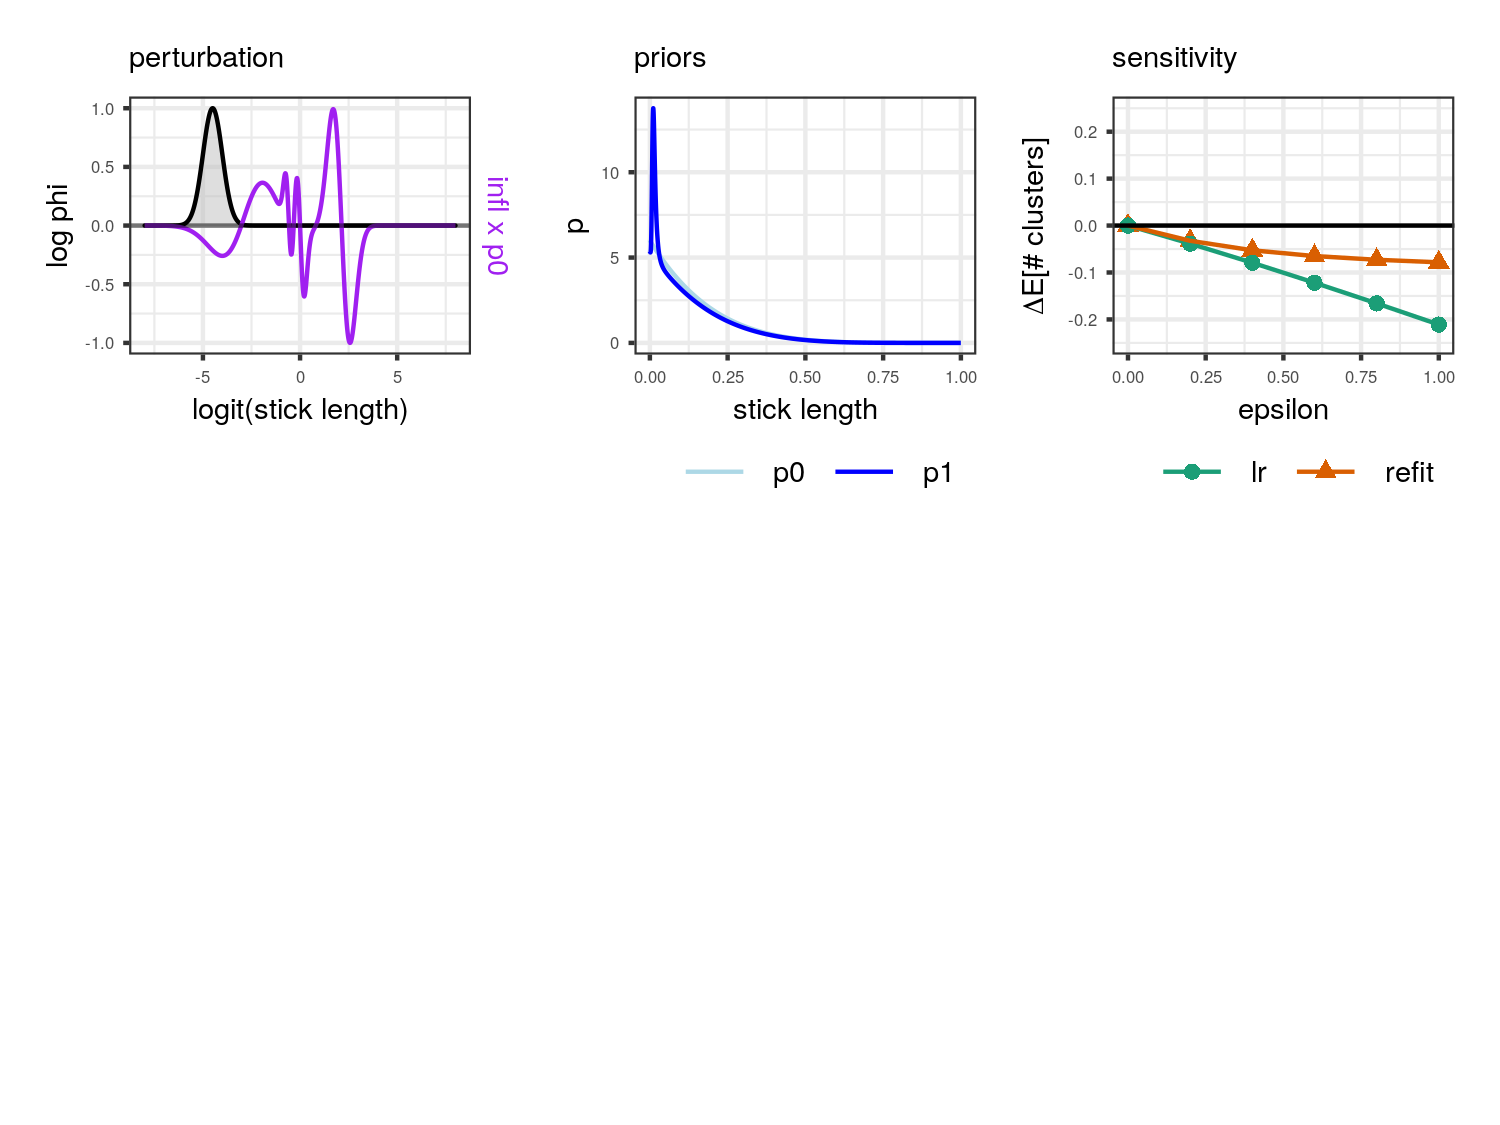
\includegraphics[width = \textwidth]{./figures/iris_func_sens0.png}}
    \only<2>{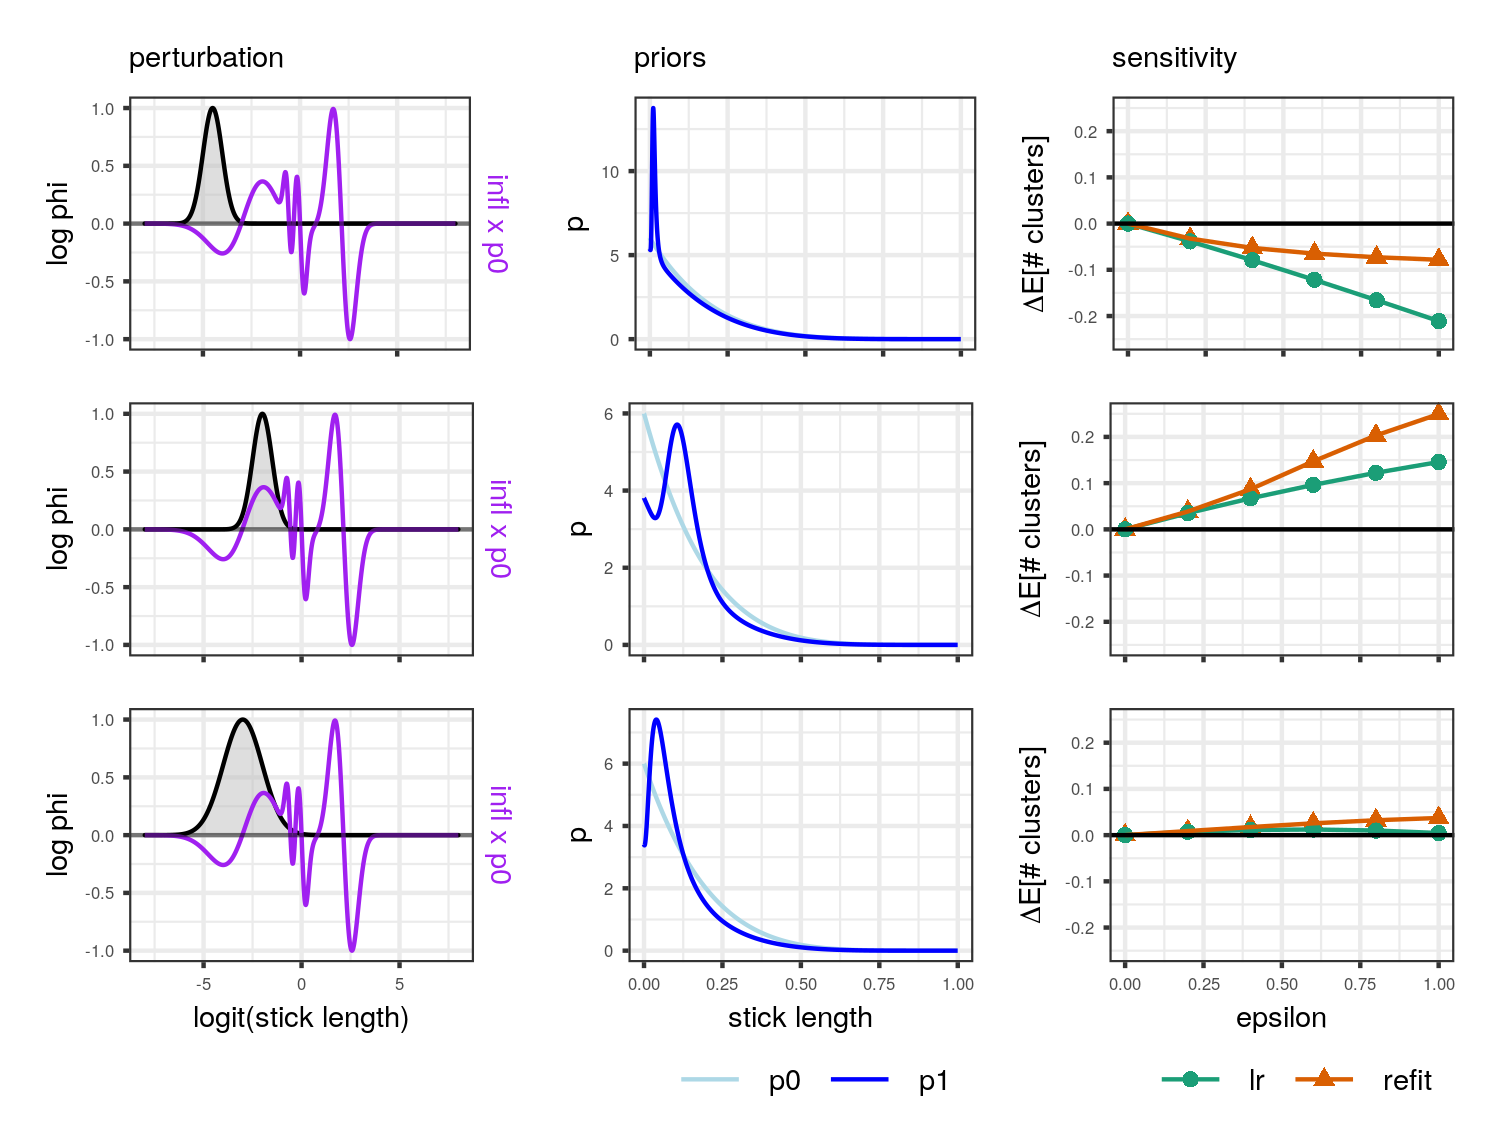
\includegraphics[width = \textwidth]{./figures/iris_func_sens1.png}}
\end{figure}
\end{frame}


\begin{frame}{iris data: worst-case perturbation}
  \begin{figure}[!h]
    \centering
    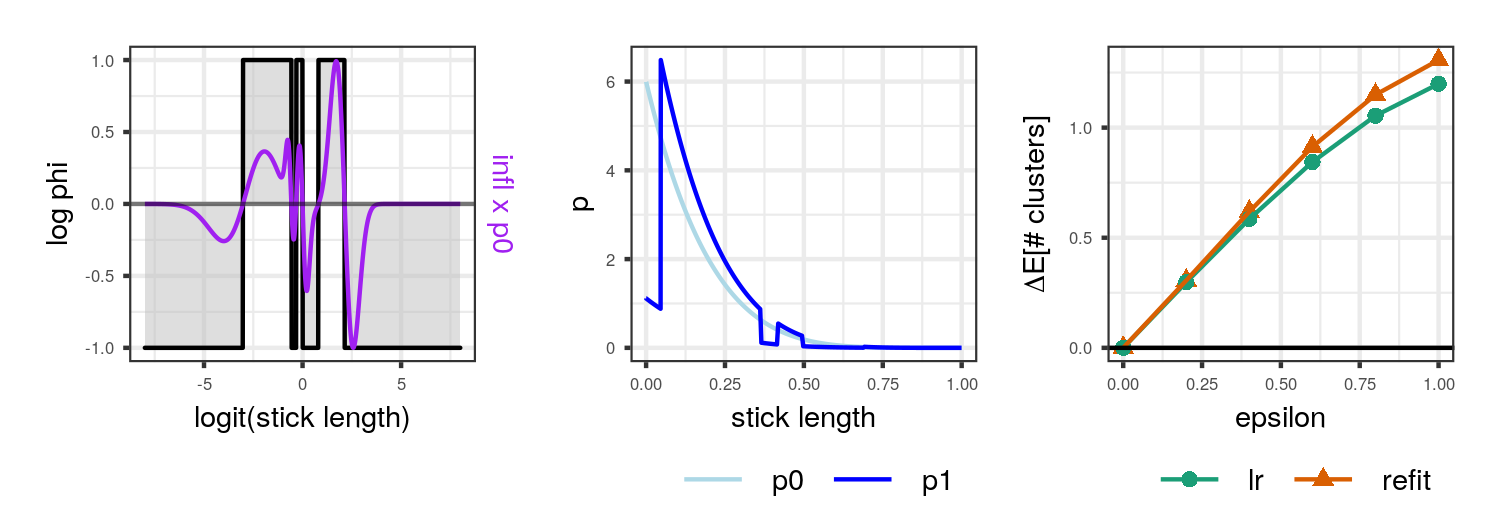
\includegraphics[width = \textwidth]{./figures/iris_worst_case.png}
\end{figure}
\end{frame}


\begin{frame}{Results on fastSTRUCTURE \citep{raj:2014:faststructure}}

We adapt fastSTRUCTURE
% {\color{blue} \href{https://web.stanford.edu/group/pritchardlab/publications/pdfs/PritchardEtAl00.pdf}{(Pritchard et al. 2000};
% \href{https://www.genetics.org/content/197/2/573}{Raj et al. 2014)}
% },
a Bayesian model for population genetics, to include a BNP prior.


We study genetic data from the Taita thrush, an endangered bird species.
The data consists of microsatellites sequences of 155 individuals at 7 loci.

\begin{figure}[!h]
\centering
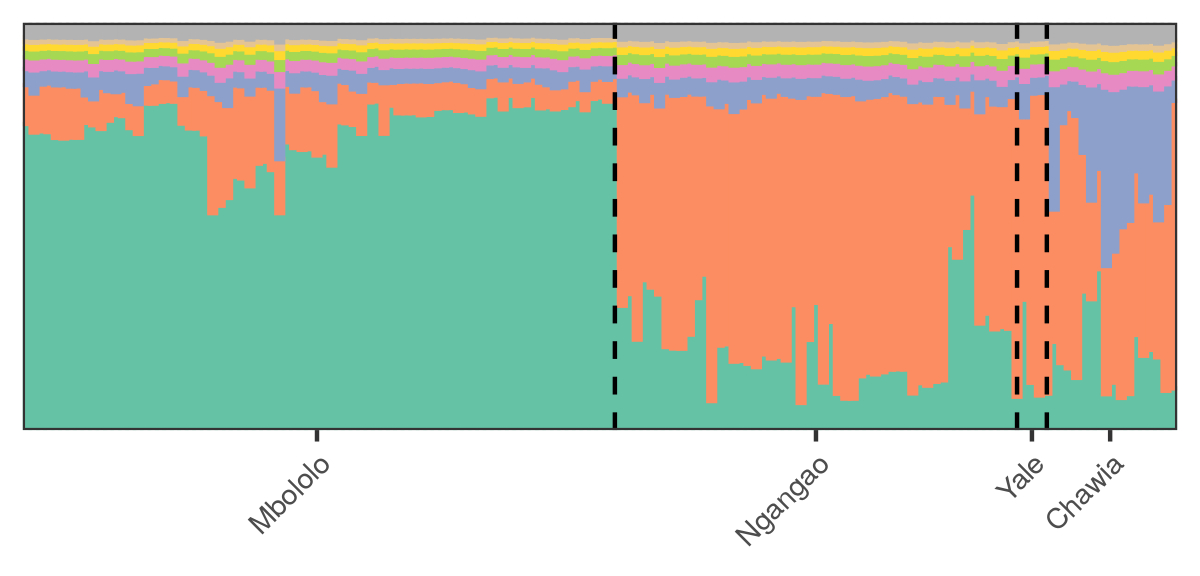
\includegraphics[width = 0.9\textwidth]{./figure/structure_init-1.png}
\caption*{The intitial fit at $\alpha = 3$. }
\end{figure}
\end{frame}


\begin{frame}{fastSTRUCTURE: Parametric Sensitivity}
  \begin{figure}[!h]
    \centering
    \only<1>{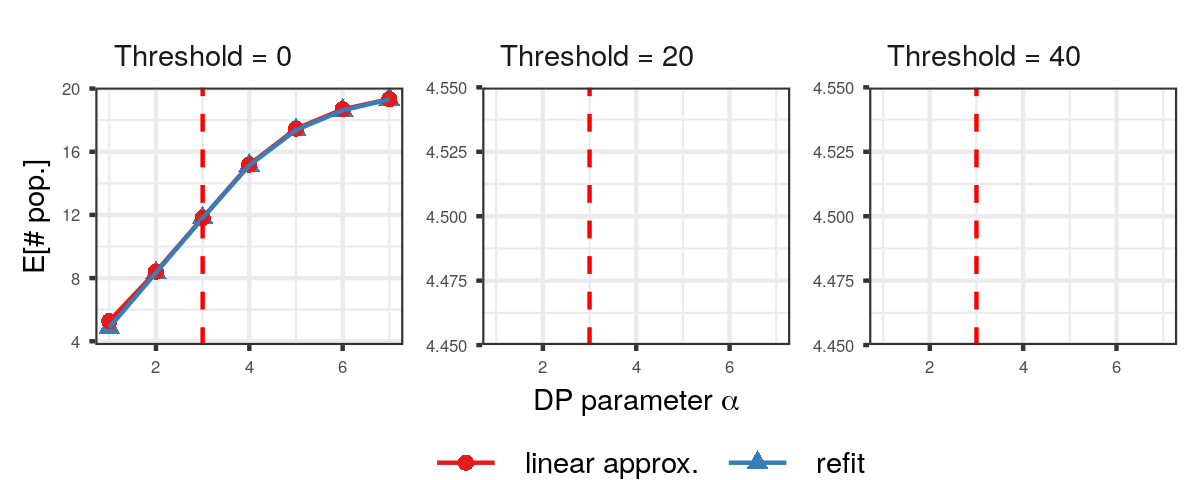
\includegraphics[width = \textwidth]{./figure/structure_alphasens0-1.png}}%
    \only<2>{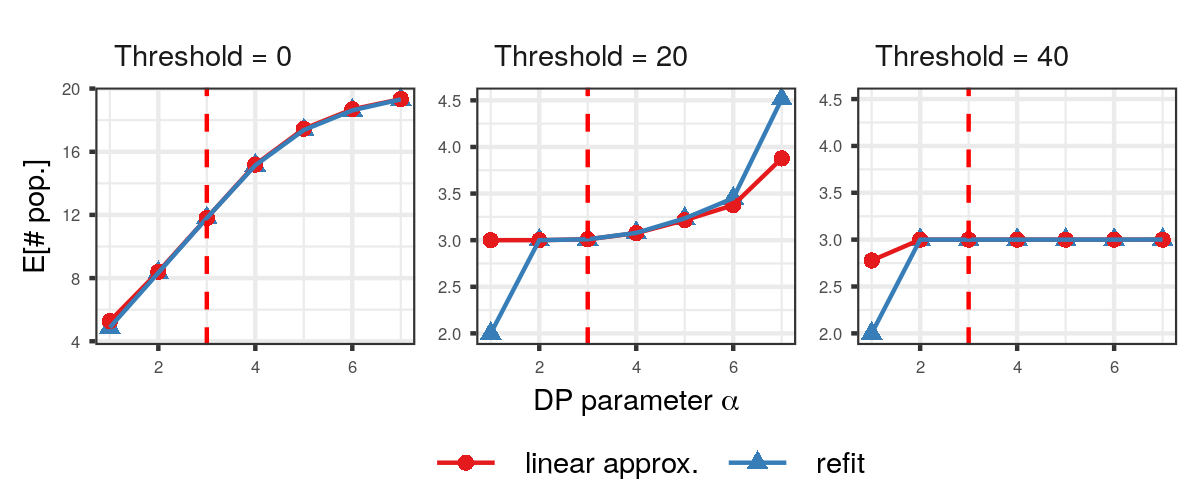
\includegraphics[width = \textwidth]{./figure/structure_alphasens-1.png}}
    \caption*{Expected number of posterior in-sample clusters in the thrush data as $\alpha$ varies.}
  \end{figure}

\end{frame}

\begin{frame}{fastSTRUCTURE: Evidence of Migration?}

  \begin{figure}[!h]
    \centering
    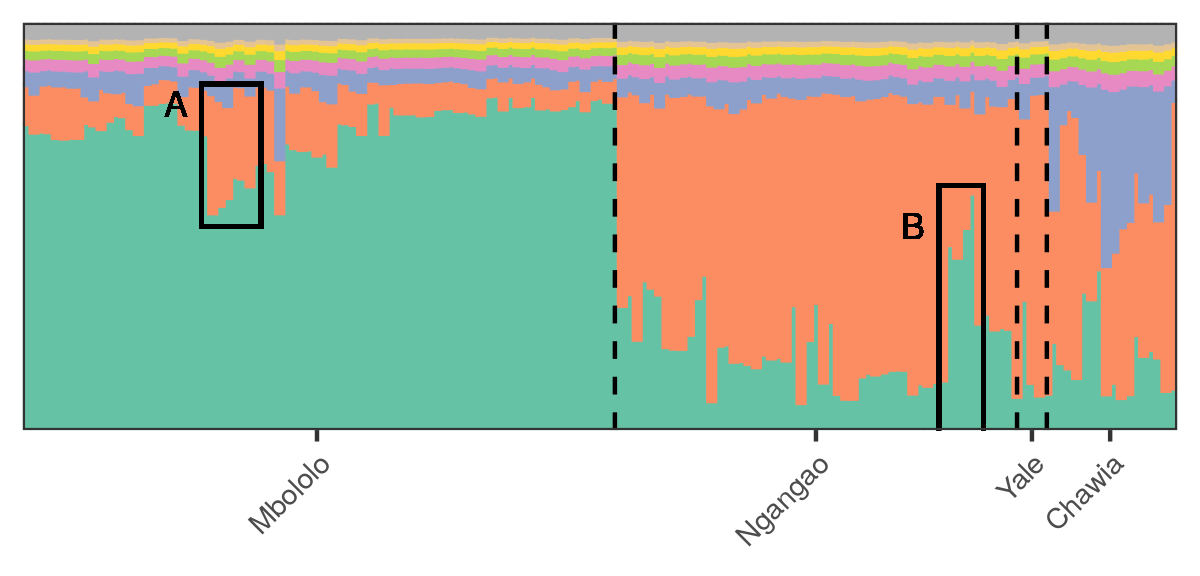
\includegraphics[width = 0.9\textwidth]{./figure/structure_migration-1.png}
  \end{figure}
\end{frame}

\begin{frame}{fastSTRUCTURE: Evidence of Migration?}
    \begin{figure}[!h]
\centering
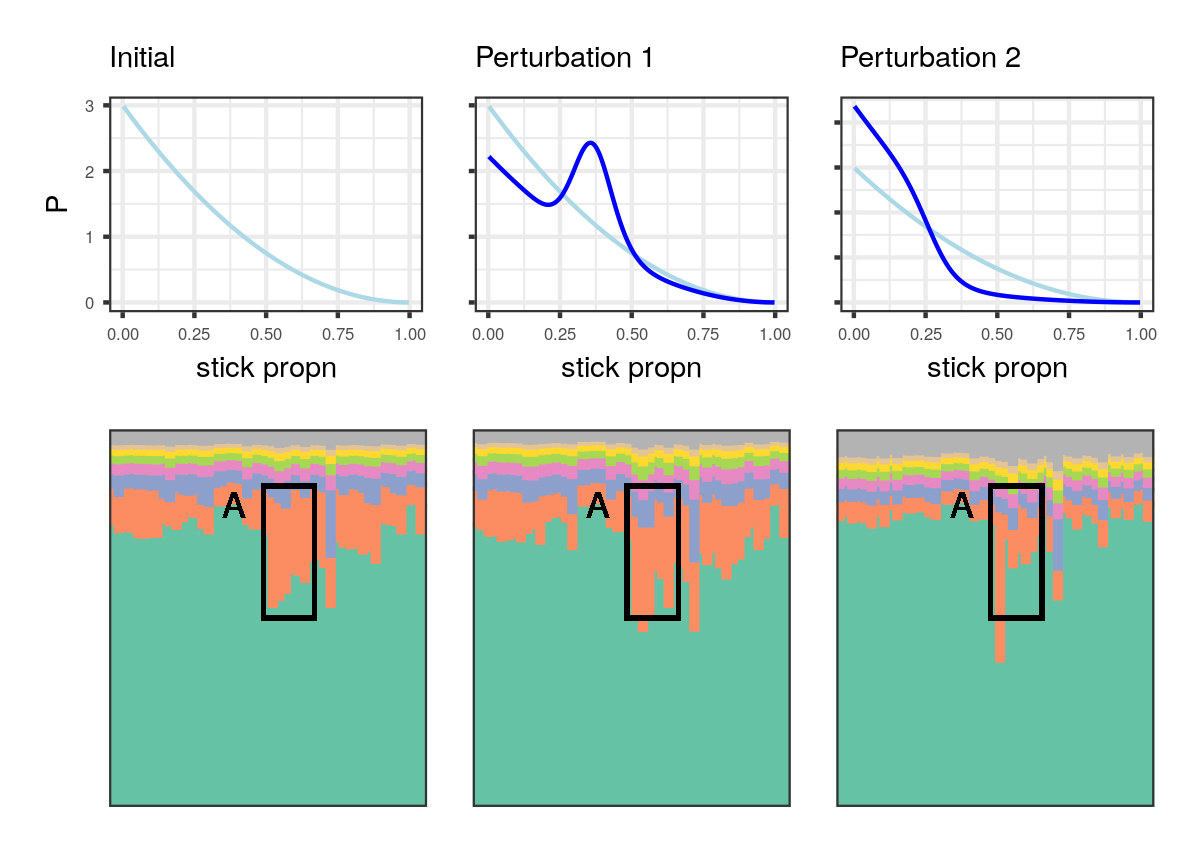
\includegraphics[width = \textwidth]{./figure/mbololo_motivating_ex-1.png}
\end{figure}

\end{frame}

\begin{frame}{fastSTRUCTURE: Functional Sensitivity}

\begin{figure}[!h]
    \centering
    \only<1>{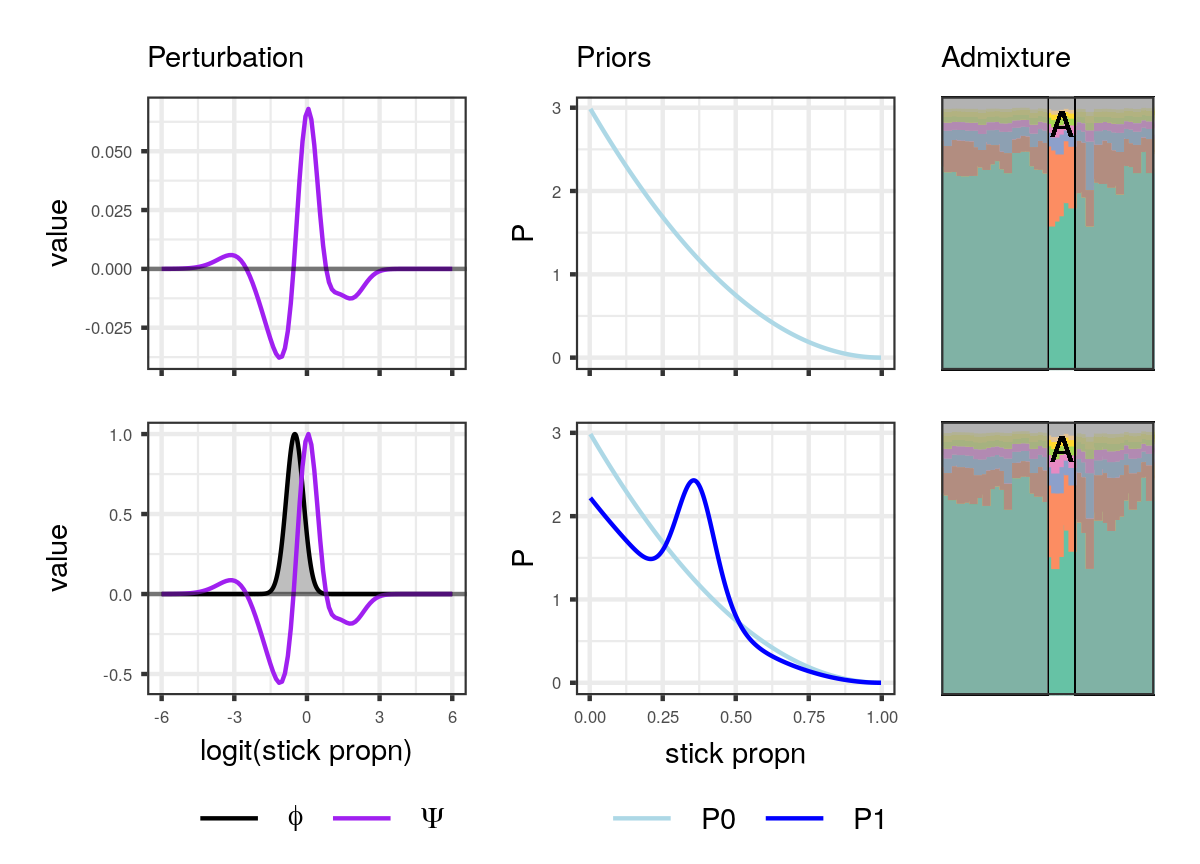
\includegraphics[width = \textwidth]{./figure/mbololo_motivating_ex_inflA-1.png}}
    \only<2>{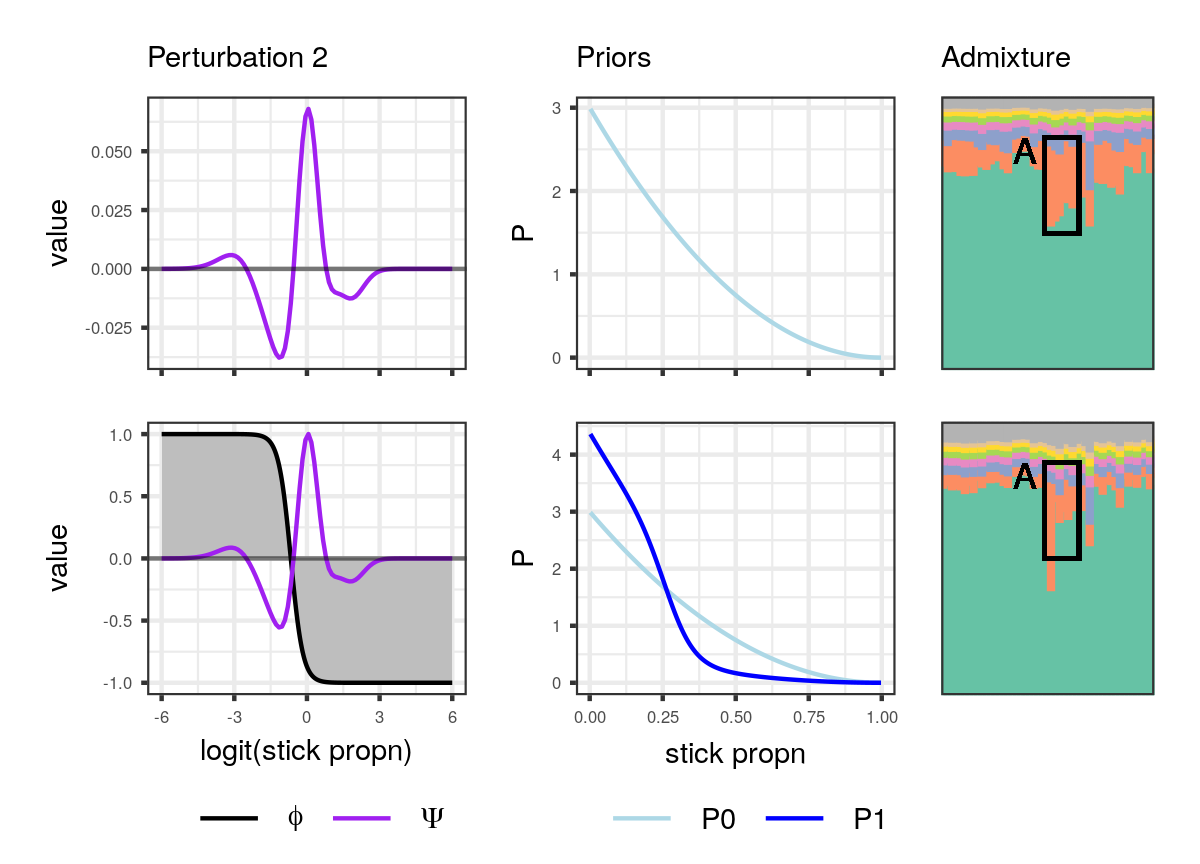
\includegraphics[width = \textwidth]{./figure/mbololo_motivating_ex_inflB-1.png}}
\end{figure}

\end{frame}

\begin{frame}{fastSTRUCTURE: Functional Sensitivity}

  \begin{figure}[!h]
    \centering
    \only<1>{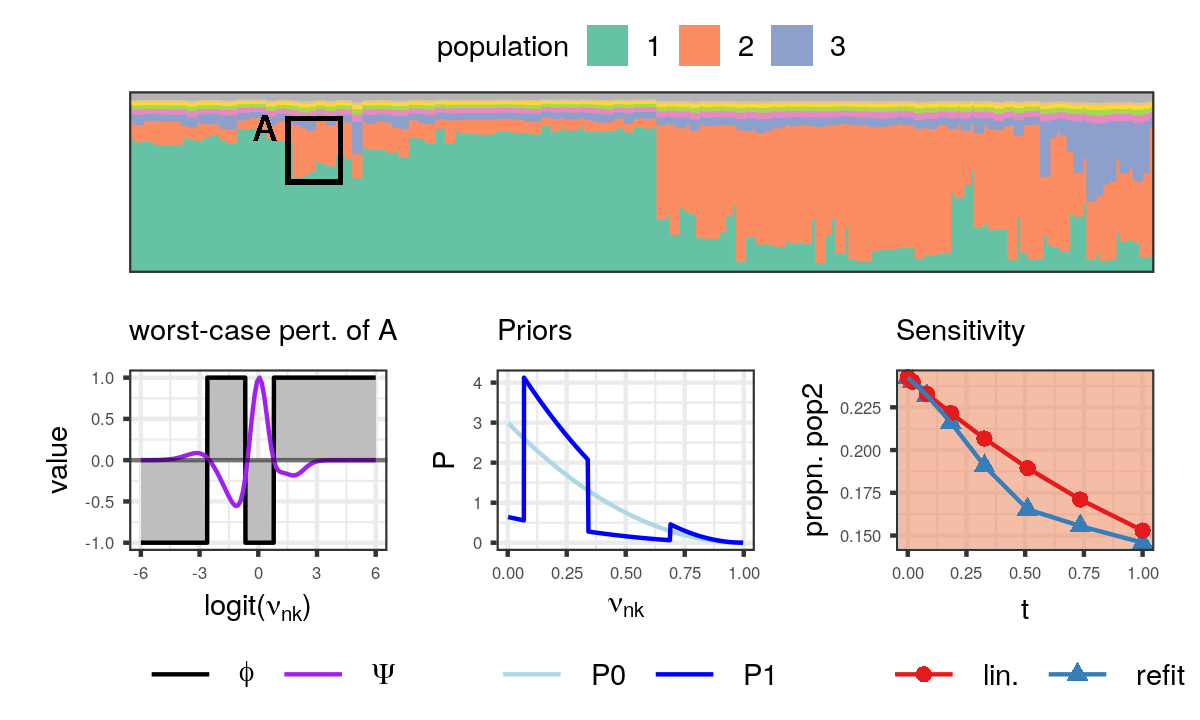
\includegraphics[width = \textwidth]{./figure/mbololo_outliers-1.png}}%
    \only<2>{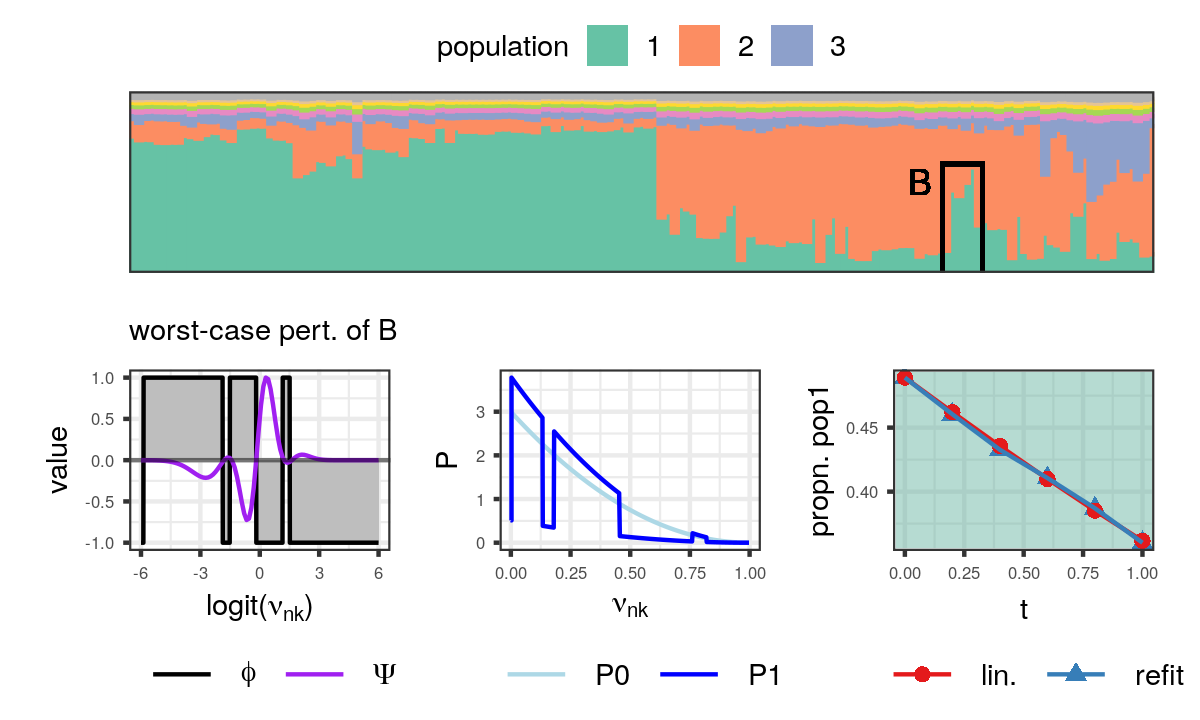
\includegraphics[width = \textwidth]{./figure/ngangao_outliers-1.png}}%
    % \only<3>{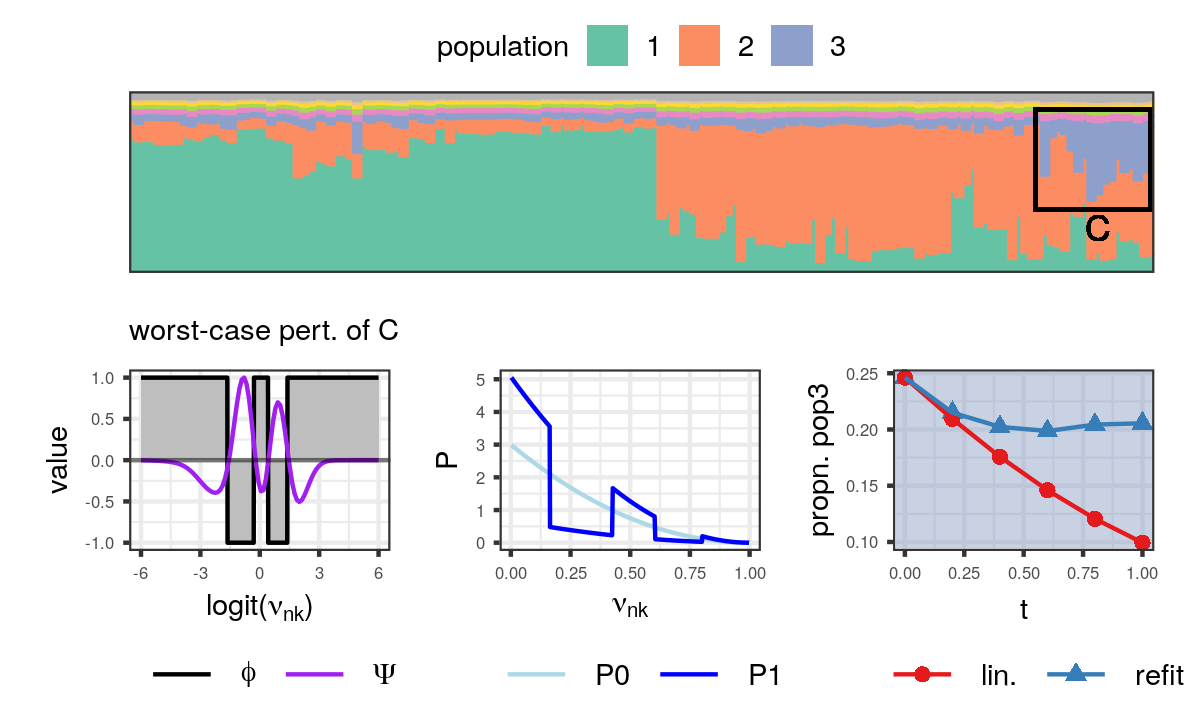
\includegraphics[width = \textwidth]{./figure/chawia_outliers-1.png}}
  \end{figure}

\end{frame}

%%%%%%%%%%%%%%%%%%%
% limitations of local sensitivity
%%%%%%%%%%%%%%%%%%%


\begin{frame}{Limitations of Local Sensitivity}
  \begin{figure}[!h]
    \centering
    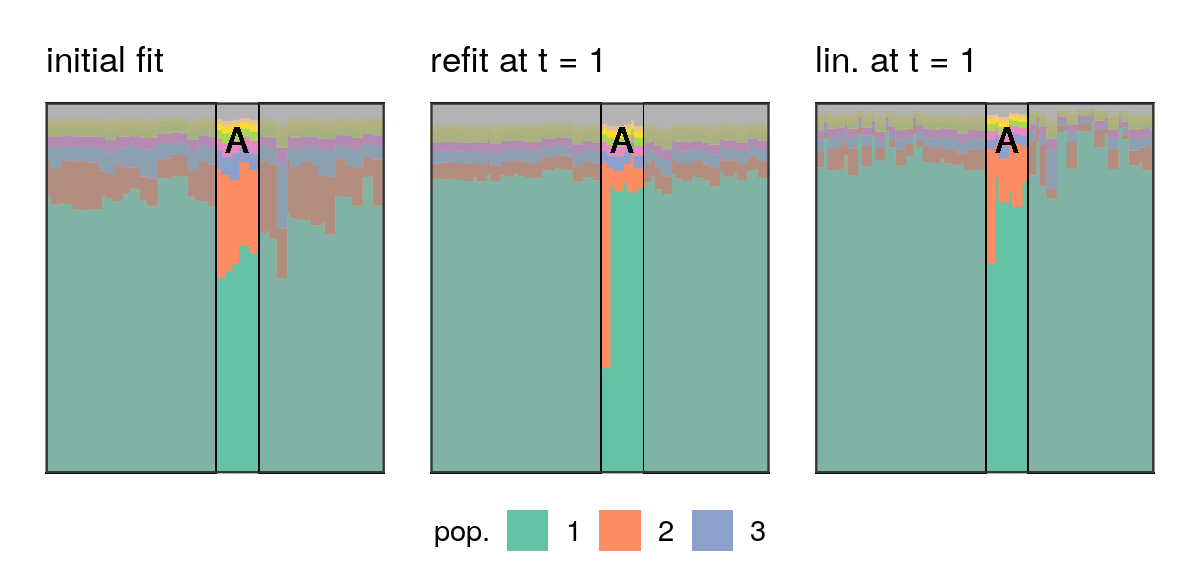
\includegraphics[width = \textwidth]{./figure/bad_admix_ex-1.png}
    \caption*{Inferred admixtures after the worst-case perturbation
     to individuals A.
     Individual $n = 26$ had a large increase in admixture proportion of
     population 2 after the refit. }
  \end{figure}

\end{frame}

\begin{frame}{Limitations of Local Sensitivity}

  \begin{figure}[!h]
    \centering
    \only<1>{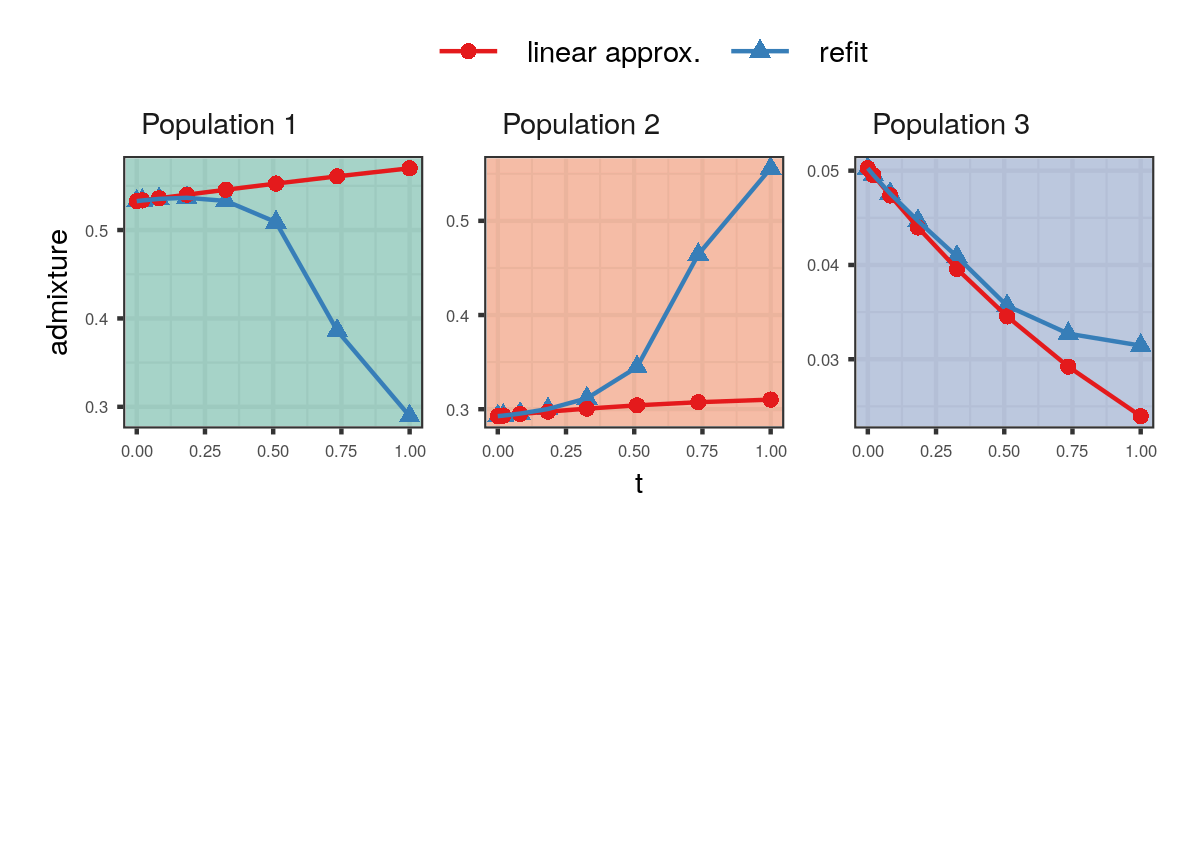
\includegraphics[width = \textwidth]{./figure/bad_admix_trace_admix-1.png}}%
    \only<2>{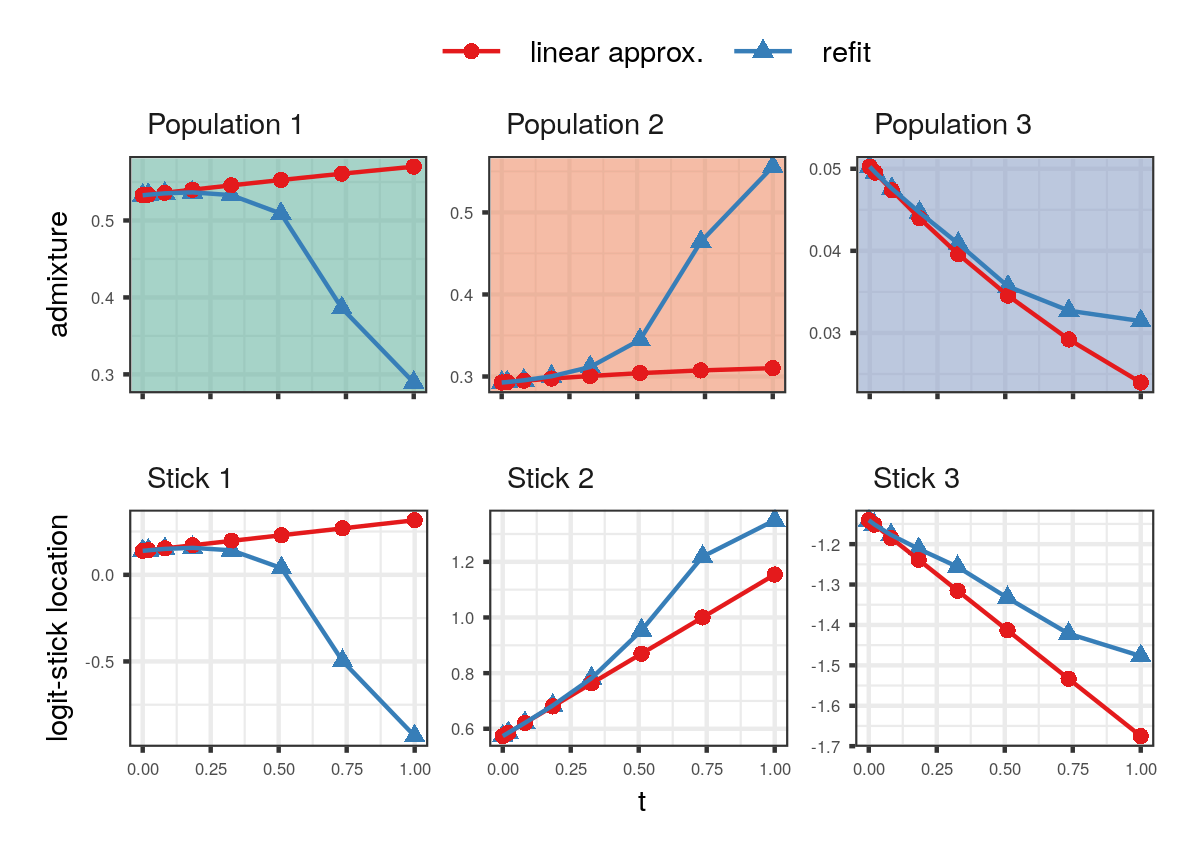
\includegraphics[width = \textwidth]{./figure/bad_admix_trace_all-1.png}}%
  \end{figure}

\end{frame}

\begin{frame}{Computational Complexity}

\begin{table}[tb]
\centering
\caption*{Compute time of results on the Taita thrush dataset. }
\begin{tabular}{|r|r|}
\hline
    & time (seconds) \\
    \hline
    Initial fit & 7 \\
    \hline
    Hessian solve for $\alpha$ sensitivity & 0.3\\
    Linear approx. $\eta^{lin}(\alpha)$ for $\alpha = 1, ..., 7$ &
        0.006 \\
    Refits $\eta(\alpha)$ for $\alpha = 1, ..., 7$ &
        30 \\
    \hline
    The influence function & 0.6 \\
    Hessian solve for perturbation $\phi$ &
        0.4 \\
    Linear approx. $\eta^{lin}(\epsilon)|_{\epsilon = 1}$
      for perturbation $\phi$ &
        0.001\\
    Refit $\eta(\epsilon)|_{\epsilon = 1}$
      for perturbation $\phi$ &
        10 \\
    \hline
\end{tabular}
\end{table}



\end{frame}


\begin{frame}{Summary}

\vspace{1em}

\begin{mdframed}[style=MyFrame]
\begin{center}
{\bf Our linear approximation provides a fast and reasonable alternative to
re-evaluating the full model after changing the BNP prior.}
\end{center}
\end{mdframed}

\vspace{0.5em}

{\bf A related workshop paper: }\newline
Runjing Liu, Ryan Giordano, Michael I. Jordan, Tamara Broderick. \newline
“Evaluating Sensitivity to the Stick Breaking Prior in Bayesian Nonparametrics.”
\newline {\color{blue}\url{https://arxiv.org/pdf/1810.06587.pdf}}

\vspace{1em}

{\bf Code: }\newline
Paragami: parameter folding and flattening for optimization problems \newline
{\color{blue}\url{https://github.com/rgiordan/paragami}}

Vittles: library for sensitivity analysis in optimization problems \newline
{\color{blue}\url{https://pypi.org/project/vittles/}}


\end{frame}


\end{document}

% \begin{frame}{Functional perturbations: worst case}
%
% There are many possible choices for $p_1$.
% We consider the {\itshape worst-case} perturbation.
%
% \pause
%
% Define the inner-product,
% \begin{align*}
%     \langle a, b\rangle := \int a(\nu)b(\nu)p_0(\nu)\lambda(d\nu).
% \end{align*}
%
% Let $\phi(\nu) := \log p_1(\nu) - \log p_0(\nu)$.
% Then the sensitivity can be written as
% \begin{align*}
% \frac{d \eta^*(\epsilon)}{d\epsilon^T}\Big|_{\epsilon=0}
%  &= \langle \mathcal{I}, \phi\rangle,
% \end{align*}
% $\mathcal{I}$ being the {\itshape influence function}.
% We can view $\mathcal{I}$ as a functional derivative (in an appropriate norm).
%
% \end{frame}
%
% \begin{frame}{Results: functional perturbation}
% The worst-case perturbation is defined as
% \begin{align*}
%   \text{arg\,sup}\Big\{\langle \mathcal{I}, \phi\rangle :
%         \phi \in B_\delta \Big\},
% \end{align*}
% $B_\delta$ a ball of radius $\delta$ in some norm.
%
% \vspace{-1em}
%
% \begin{figure}[!h]
% \centering
% 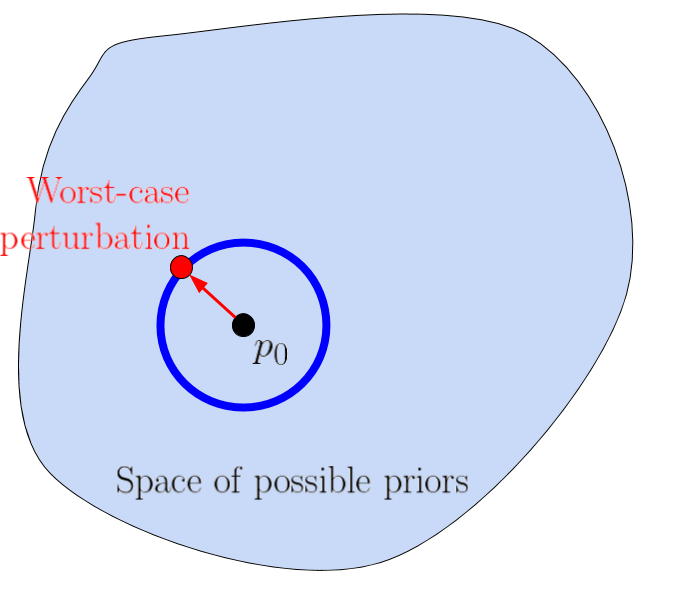
\includegraphics[width = 0.4\textwidth]{./images/functional_perturbation_worst_case.png}
% \setlength{\textfloatsep}{-10pt}
% \end{figure}
%
% If $B_\delta$ is the L-infinity-ball of radius $\delta$, then
% the worst-case $\phi^*$ is given by
% \begin{align*}
%   \phi^*(\nu) = \delta \cdot \text{sign}(\mathcal{I}(\nu))
% \end{align*}
%
% \end{frame}
